\documentclass[10pt]{article}

%gestion du français et des accents
\usepackage[utf8]{inputenc}
\usepackage[T1]{fontenc}
\usepackage[french]{babel}

%symbole mathématique
\usepackage{amsmath}
\usepackage{amsthm}
\usepackage{amssymb}
\usepackage[colorlinks=true, linkcolor=blue, urlcolor=blue]{hyperref}
\usepackage{bm}
\usepackage{amscd} 
\usepackage{tabularx}
\usepackage{stmaryrd}
\usepackage{cleveref}
\usepackage{mathdots}
\usepackage{siunitx}
\usepackage{wrapfig}





%mise en page
\usepackage[margin=1in]{geometry}
\usepackage{lmodern}
%\usepackage{mathrsfs}
\usepackage{fancyhdr}
\usepackage{soul}
\usepackage{float}
\usepackage{titlesec}
\usepackage{enumitem}
\usepackage{tcolorbox}
\usepackage{graphicx}
\usepackage{caption}
\usepackage{xcolor}

\pagestyle{fancy}    % Utiliser un style d'en-têtes personnalisés
\fancyhf{}           % Réinitialise les en-têtes et pieds de page
\fancyhead[L]{Anthony Gabino}  % Nom de l'auteur à gauche
\fancyhead[R]{\nouppercase{\leftmark}}  % Titre du sous-chapitre à droite
\fancyfoot[C]{\thepage}  % Numéro de page centré en bas
\setcounter{tocdepth}{2}

\numberwithin{equation}{section}

%configuration des sections et sous-sections
\titleformat{\subsection}[block]   % format "block"
{\centering\large\bfseries}      % centrage + taille + gras
{\thesubsection}                 % numéro de la sous-section
{1em}                            % espace entre numéro et texte
{}  

\titleformat{\section}    % section = "Chapitre"
[block]                 % format en bloc
{\centering\large}      % style : centré, grand (pas en gras)
{\MakeUppercase{Chapitre \thesection}} % numéro en majuscules
{0pt}                   % pas d’espace entre numéro et texte
{\vspace{1ex}\\\bfseries\huge}  % saut de ligne + texte en énorme

\titlespacing*{\section}{0pt}{3.5ex plus 1ex minus .2ex}{10ex} 

\newcommand{\norme}[1]{ \left\| #1 \right\|}

\newcommand{\et}{\quad \text{et} \quad}

\newcommand{\ou}{\quad \text{ou} \quad}

\begin{document}
	\begin{titlepage}	
		\thispagestyle{empty}
		\vspace*{-2.5cm}
		\mdseries{
			
			\begin{center}
				\includegraphics[width=0.35\textwidth]{"logo-epfl.png"}
				
				{\Large
					\textsc{École Polytechnique Fédérale de Lausanne }}\\
				\rule{11cm}{1pt}
				
				
				\vspace*{7cm} 
				
				{\fontsize{47}{47} \selectfont
					Physique II}\\
				\vspace*{0.5cm}
				{PHYS-108}
				
				
				\vspace*{1.5truecm} 
				
				{\small
					Note de  
				}
				
				{\large
					\vspace*{0.3cm}
					Anthony Gabino
				}
			\end{center}
			
			\vspace*{2cm}
			
			\begin{tabular}{@{}ll}
				\small
				Professeur :\\[0.5cm]
				\normalsize
				\quad Christian Theiler & \hspace{3.1cm}%..............................\\[0.1cm]
			\end{tabular}
			
			\vspace*{1.0truecm}
			
			\begin{center}
				\rule{3cm}{1pt}
				\vspace*{0.5cm}
				
				\small
				Dernière mise à jour \today\\
				Bachelor Mathématique\\
				Lausanne
			\end{center} 
			
			\clearpage
		}
	\end{titlepage}
	\tableofcontents
	
	\clearpage
	
	\section{Notations et mathématique de base}
	\subsection{Scalaires et vecteurs}
	On distinguera les quantités \emph{scalaires} et les quantités \emph{vectorielles}. Dans un repère cartésien en trois dimension, on a
	\[
	\bm u = u_x \bm e_x + u_y \bm e_y + u_z \bm e_z \ou \bm u = (u_x, u_y, u_z)
	\]
	on définit alors la \emph{norme} de $\bm u$ comme 
	\[
	u = \norme{\bm u} = \sqrt{u_x^2 + u_y^2 + u_z^2} 
	\]
	Souvent les quantités scalaires et vectorielles sont une fonction de la position $\bm r$ et du temps $t$. On parle alors de \emph{champs scalaires} et \emph{champs vectoriels}, que l'on note
	\[
	f(\bm r, t) \et \bm u(\bm r, t)
	\]
	\subsection{Opérateur $\nabla$}
	En coordonnées cartésiennes, le \emph{vecteurs opérateurs} $\nabla$ est définit par
	\[
	\nabla = (\partial_x, \partial_y, \partial_z)
	\]
	où $\partial_x = \frac{\partial}{\partial x}$ correspond à la dérivée partielle par rapport à $x$. Ainsi le \textbf{gradient} $\nabla f$ d'un champ scalaire $f$ est le champ vectoriel
	\[
	\boxed{\nabla f(\bm r, t) = \frac{\partial f}{\partial x} \bm e_x + \frac{\partial f }{\partial y} \bm e_y + \frac{\partial f}{\partial z} \bm e_z}
	\]
	Le gradient $\nabla f$ est perpendiculaire aux isosurface et est dirigé dans la direction d'aumgmentation de $f$.
	
	La \textbf{divergence} $\nabla \cdot \bm u$ d'un champ vectoriel $\bm u$ est le champ scalaire
	\[
	\boxed{\nabla \cdot \bm u( \bm r, t) = \frac{\partial u_x}{\partial x} \bm e_x + \frac{\partial u_y}{\partial y} \bm e_y + \frac{\partial u_z}{\partial z} \bm e_z}
	\]
	la divergence $\nabla \cdot \bm u$ permet de quantifier, localement, la variation du gradient, c'est-à-dire su le champ se comporte comme une source ou comme un puit.
	
	Finalement, le \textbf{rotationel} $\nabla \times \bm u$ d'un champ vectoriel est le champ vectoriel
	\[
	\boxed{
	\nabla \times \bm u(\bm r, t) = \left(\frac{\partial u_z}{\partial y} - \frac{\partial u_y}{\partial z} \right) \bm e_x + \left( \frac{\partial u_x}{\partial z} - \frac{\partial u_z}{\partial x} \right) \bm e_y + \left( \frac{\partial u_y}{\partial x } - \frac{\partial u_x}{\partial y} \right) \bm e_z}
	\]
	Le rotationel $\nabla \times \bm u$ exprime la tendant qu'ont les lignes de champ à tourner autour d'un point.
	
	Les opérateurs différentiels comme le gradient, la divergence ou le rotationnel décrivent des variations locales d'un champ, au voisinage d'un point. On souhaite pouvoir connaître l'effet net du phénomène au bord afin de comprendre la totalité des variations internes de ce même phénomène et vice-versa.
	
	\subsubsection*{Théorème du gradient}
	Soit $f$ un champ scalaire continûment dérivable sur un volume $V$ dont le bord est noté $S := \partial V$. Alors
	\[
	\boxed{\iint_S f \mathrm d \bm S = \iiint_V \nabla f \mathrm d V}
	\] 	
	où $\mathrm d \bm S$ est le vecteur \emph{élément de surface} perpendiculaire à la surface $S$ vers l'extérieur avec $\norme{\mathrm d \bm S} = \mathrm d S$.
	
	\subsubsection*{Théorème de la divergence}
	On définit le \emph{flux} d'un champ vectoriel $\bm u$ à travers une surface $S$ par 
	\[
	\Phi = \iint_S \bm u \cdot \mathrm d \bm S
	\]
	Le flux mesure alors la quantité de champ par unité de temps qui traverse la surface $S$. Ainsi, soit $\bm u$ un champ vectoriel continûment dérivable sur un volume $V$ de bord $S = \partial V$, alors
	\[
	\boxed{\Phi = \iint_S u \cdot \mathrm d \bm S = \iiint_V \nabla \cdot \bm u ~\mathrm d V}
	\]
	
	\subsubsection*{Théorème de Stokes}
	On définit la \emph{circulation} d'un champ vectoriel $\bm u$ le long d'une courbe fermée $\Gamma$ comme
	\[
	\Sigma = \oint_\Gamma \bm u \cdot \mathrm d \bm l
	\]
	où $\mathrm d \bm l$ est tangent à la courbe et orienté dans le sens de rotation. Ainsi, soit $\bm u$ un champ vectoriel continûment dérivale sur une surface de borde $\partial S = \Gamma$, alors
	\[
	\boxed{\Sigma = \oint_\Gamma \bm u \cdot \mathrm d \bm l = \iint_S \left(\nabla \times \bm u\right) \cdot \mathrm d \bm S}
	\]
	Autrement dit, la rotation globale observée sur le bord provient de l'accumulation des rotations internes.
	\clearpage
	\section{Fluides au repos}
	\subsection{Définition de vase}
	Un fluide peut être décrit par la \emph{densité de masse} $\rho(\bm r, t)$, la \emph{pression} $p(\bm r, t)$ et la vitesse \emph{vitesse} $\bm u(\bm r, t)$. Dans ce chapitre on supposera que
	\[
	\bm u(\bm r, t) = \bm 0, \quad \rho(\bm r, t) = \rho(\bm r), \quad p(\bm r, t) = p(\bm r)
	\]
	On peut alors définie ces grandeurs formellement. Ainsi, la \emph{densité} au point $\bm r$ est donnée par
	\[
	\boxed{\rho(\bm r) = \left.\lim_{\Delta V \to \mathrm d V} \frac{\Delta m}{\Delta V} \right|_{\bm r} }
	\]
	avec $[\rho] = \mathrm{kg} \cdot \mathrm m^{-3}$. On peut définir la \emph{masse} d'un volume de fluide comme
	\[
	m = \iint_V \rho(\bm r) \mathrm dV
	\]
	La deuxième grandeur scalaire est la \emph{pression} définit comme la force par unité de surface exercée par le fluide. Cette force est perpendiculaire à la surface,
	\[
	\mathrm d \bm F = p \mathrm d \bm S
	\]
	avec $[p] = \mathrm N \cdot \mathrm m^{-2} = \mathrm{Pa}$. Puisque la pression est isotrope, alors on a bien un champ scalaire.
	
	\subsection{Pression hydrostatique}
	
	\begin{minipage}{0.6\textwidth}
		Si on considère un fluide incompressible, c'est-à-dire $\rho(\bm r) = cste$, alors
	\[
\boxed{
	p(h) = p_0 + \rho g h}
\]
En effet puisque le fluide est au report,
\[
\bm 	F_1 + \bm F_2 + \bm F_p = \bm 0
\]
donc par définition de celles-ci
\[
p(z_1)  \mathrm d x \mathrm dy + \rho g \mathrm d x \mathrm d y (z_2 - z_1) + p(z_2) \mathrm d x \mathrm d y =  0
\]
ce qui nous donne $p(z_2) = p(z_1) + \rho g (z_2 - z_1)$. En particulier, pour $z_1 = 0$ et $z_2 = h$, on a bien
\[
p(h) = p_0 + \rho g h
\]
\vspace{0.5cm}
\end{minipage}
\hfill
\begin{minipage}{0.4\textwidth}
	\centering
	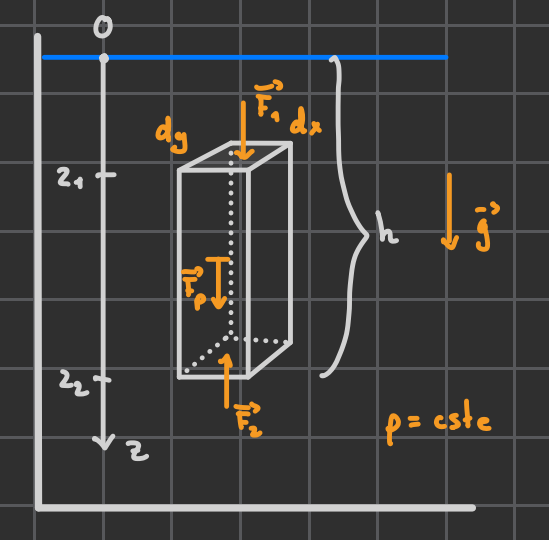
\includegraphics[width=0.8\textwidth]{images/pression-hydrostatique.png}
	\captionof{figure}{Pression hydrostatique}	
	\vspace{0.5cm}
\end{minipage}

 Si on considère un corps de volume $V$ plongé dans un fluide au repos alors il subit une force verticale, dirigée de bas en haut,
 \[
 \boxed{\bm P_A = - \rho V \bm g}
 \]
 On l'appelle la \emph{poussée d'Archimède}. En effet dans le cadre pression hydrostatique $p = p_0 - \rho g z$, par le théorème du gradient
 \[
 \bm P_A = - \iint_S p \mathrm d \bm S = \iint_V - \nabla p \mathrm d V = \iiint_V - \nabla (p_0 - \rho g z) \mathrm d V = \rho g \iiint_V \mathrm d V \bm e_z = \rho V g \bm e_z = - \rho V \bm g
\]
\subsection{Tension superficielle}

\subsubsection{Définition de base}
Si on considère une interface de contact liquide-gaz de longueur $L$, alors
\[
\boxed{
F_\gamma = \gamma L}
\]
est la \emph{force de tension superficielle}. Cette force est tangentielle à l'interface et perpendiculaire à sont bord. La \emph{tension superficielle} correspond donc à la force qu'il faut exercer pour augmenter la surface d'un système. De plus
\[
\boxed{\Delta W = \gamma \Delta S}
\]

\subsubsection{Loi de Young}
\begin{minipage}[L]{0.4\textwidth}
	\centering
		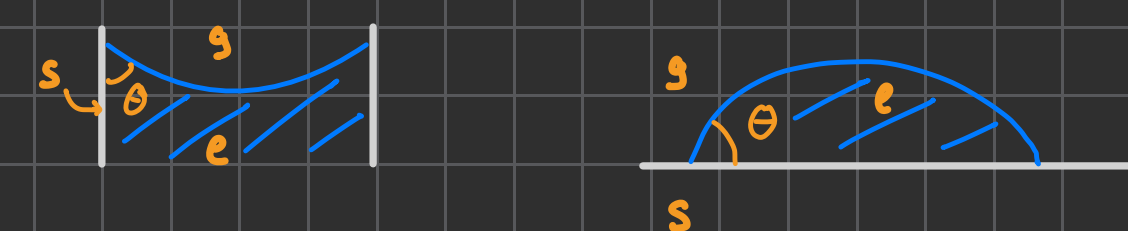
\includegraphics[width=0.8\textwidth]{images/angle-contact.png}
		\captionof{figure}{Angle de contact}
\end{minipage}
\hfill
\begin{minipage}[L]{0.6\textwidth}
Si on se place dans le cadre d'une interface solide-liquide-gaz, alors
\[
\boxed{\cos \theta = \frac{\gamma_{sg} - \gamma_{sl}}{\gamma_{gl}}}
\]
où $\theta$ correspond à l'angle de contact statique comme ci-près.
\end{minipage}

\subsubsection{Loi de Laplace}
\begin{minipage}{0.6\textwidth}
	Si on considère dès une surface sphèrique, comme ci-près, on remarque alors qu'au voisinage de $M$, la surface $S$ est assimilable à une surface d'ellipse de courbure principale $R_1$ et $R_2$, où $R_1 \leqslant R_2$, ainsi on 
	\[
	\boxed{p_1 = p_2 + \gamma \left(\frac1{R_1} + \frac1{R_2} \right)}
	\]
	\end{minipage}
	 \hfill
\begin{minipage}{0.4\textwidth}
	\centering
	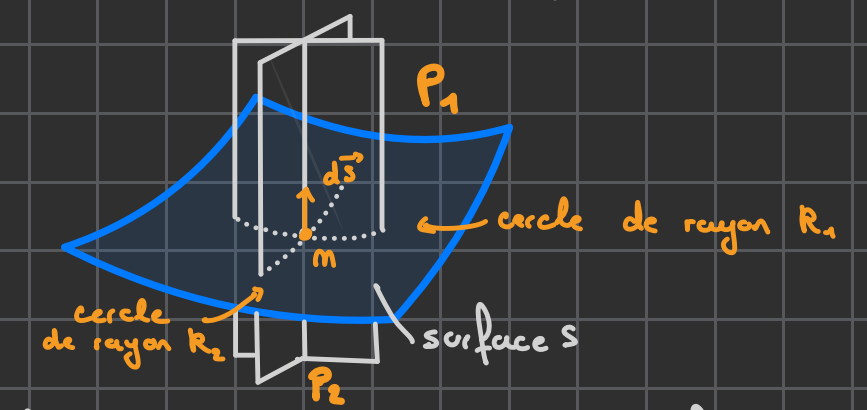
\includegraphics[width=0.8\textwidth]{images/loi-de-Laplace.png}
	 \captionof{figure}{Loi de Laplace}
\end{minipage}

\subsubsection{Loi de Jurin}
On considère que l'interface liquide-gaz est sphérique donc par Laplace la pression du à la tension superficielle est donnée par $\Delta p = \frac{2\gamma}{R}$ or comme on est à l'équilibre cette sous pression est compenser par $\Delta p = \rho g h$, ainsi 
\[
\boxed{h = \frac{2 \gamma}{\rho g R} = \frac{2 \gamma \cos \theta}{\rho g r} \propto \frac1r}
\]
ainsi la hauteur de capillarité est inversement proportionnel au rayon $r$ du tube.

\clearpage
\section{Dynamique des fluides}

\subsection{Dérivée convective}
On considère dès lors un fluide en mouvement, on les décrit par les champs scalaires et vectoriel suivants
\[
\rho(\bm r, t), \quad p(\bm r, t) , \quad \bm u(\bm r, t)
\]
où $\bm u(\bm r, t)$ est la vitesse d'éléments de fluide infinitésimales. On définit alors la \emph{dérivée convective} comme 
\[
\boxed{\frac{\mathrm D}{\mathrm Dt} = \frac{\partial }{\partial t} + \bm  u \cdot \nabla}
\]
on remarque alors que, la première partie correspond à la variable locale tandis que la deuxième partie correspond à la variation liée au déplacement de la particule.

\subsection{Équations de fluides}
On a vu qu'un fluide en mouvement était caractérisé par $5$ fonctions
\[
\rho, \quad p , \quad \bm u
\]
il nous faut donc $5$ équations pour pouvoir les déterminer.

\subsubsection{Équation de continuité (description Eulérienne)}
\noindent
\begin{minipage}{0.6\textwidth}
	Le principe de conservation de masse peut être écrit par
	\[
	\boxed{\frac{\partial \rho}{\partial t} + \nabla \cdot (\rho \bm u) = 0} \ou \boxed{\frac{\mathrm D \rho}{\mathrm Dt} + \rho (\nabla \cdot \bm u) = 0 }
	\]
En effet on remarque que la variation de masse de $V$ n'est rien d'autre que le flux de masse à travers $S$, donc
\[
\frac{\partial }{\partial t} \iiint_V \rho(\bm r, t) ~\mathrm d V =  - \iint_S \rho (\bm r,t ) \bm u(\bm r, t) ~\mathrm d \bm S
\]
Ainsi on peut faire rentrer la dérivée partielle sous l'intégrale, et par le théorème de la divergence, on obtient
\end{minipage}
\hfill
\begin{minipage}{0.5\textwidth}
	\centering
	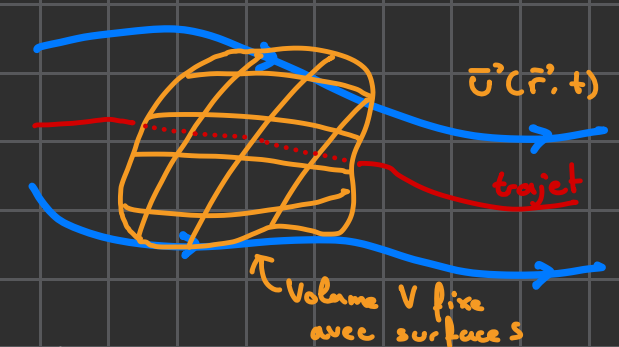
\includegraphics[width=0.8\textwidth]{images/equation-de-continuite.png}
	\captionof{figure}{Description Eulérienne}
\end{minipage}
\[
\iiint_V \frac{\partial}{\partial t} \rho(\bm r, t) \mathrm dV = - \iint_V \nabla \cdot (\rho \bm u) \mathrm d V \iff \iiint_V \left( \frac{\partial }{\partial t} \rho + \nabla \cdot (\rho \bm u) \right) \mathrm d V = 0
\]
 mais puisque $V$ est arbitraire, alors on a bien
\[
\frac{\partial \rho}{\partial t} + \nabla \cdot (\rho \bm u) = 0
\]


\subsubsection{Équation d'Euler (description Lagrangienne)}
\noindent
\begin{minipage}{0.4\textwidth}
	\centering
	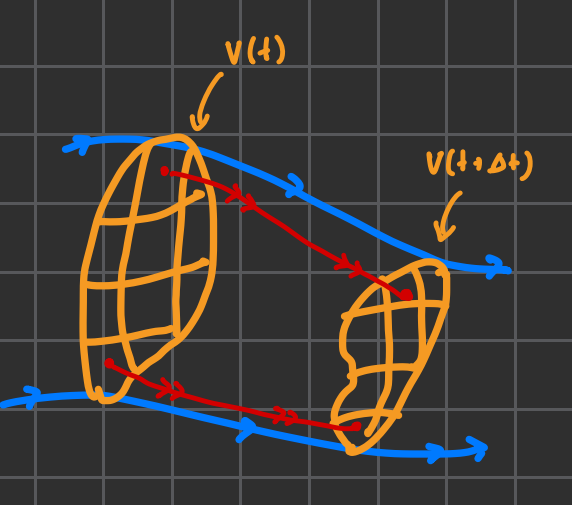
\includegraphics[width=0.8\textwidth]{images/equation-euler.png}
	\captionof{figure}{Description Lagrangienne}
\end{minipage}
\hfill
\noindent
\begin{minipage}{0.6\textwidth}
	Pour un fluide parfait, on obtient
	\[
	\boxed{\rho \frac{\mathrm D}{\mathrm Dt} \bm u = \rho \bm g - \nabla p}
	\]
	En effet, on la considère la quantité de mouvement d'un volume $V(t)$
	\[
	\bm P = \iiint_{V(t)} \rho \bm u \mathrm d V \implies \frac{\mathrm d}{\mathrm dt} \bm P = \iiint_{V(t)} \frac{\mathrm D}{\mathrm Dt}(\rho \bm u) + \rho \bm u(\nabla \cdot \bm u) \mathrm dV
	\]
	De plus par le seconde loi de Newton ($\sum \bm F = \bm{\dot P}$), donc
	\[
	\frac{\mathrm d}{\mathrm dt} \bm P = \iiint_{V(t)} \rho \bm g \mathrm dV - \iint_{S(t)} p \mathrm d \bm S = \iiint_{V(t)} (\rho \bm g - \nabla p) \mathrm dV
	\]

\end{minipage}
ainsi par identification
\[
\frac{\mathrm D}{\mathrm Dt} (\rho \bm u) + \rho \bm u(\nabla \cdot u) = \rho \bm g - \nabla p \iff \rho \mathrm{D \bm u}{\mathrm Dt} + \bm u\left( \frac{\mathrm D \rho}{\mathrm Dt} + \rho (\nabla \cdot \bm u) \right) = \rho \bm g - \nabla p
\]
on reconnait alors l'équation de continuité. On trouve donc bien l'équation souhaitée.-

\subsubsection{Équation d'état}
On considère alors un gaz parfait, alors
\[
\boxed{\frac{\mathrm D}{\mathrm Dt} (p \rho^{-\gamma}) = 0}
\]
où $\gamma$ est l'\emph{indice adiabatique}. Mais si on se place dans un liquide il est naturelle de considérer,
\[
\boxed{\rho = cste}
\]
On alors bien nos $5$ équations (on rajoute juste des conditions au bords $\bm u \cdot \mathrm d S = 0$)
\[
\frac{\partial \rho}{\partial t} + \nabla \cdot (\rho \bm u) = 0, \quad \rho \frac{\mathrm D \bm u}{\mathrm Dt} = \rho \bm g - \nabla p, \quad \frac{\mathrm D}{\mathrm Dt} (p \rho^{-\gamma}) = 0 \ou \rho = cste
\]

\subsection{Théorème de Bernoulli}
Si on considère un \emph{fluide parfait} (pas de viscosité, par de conduction de chaleur, incompressible, écoulement stationnaire ($\frac{\partial}{\partial t} = 0$). Alors le long d'une ligne de courant on a,
\[
\boxed{\frac12 \rho u^2 + \rho g z + p = cste}
\]
\noindent
\begin{minipage}{0.5\textwidth}
	En effet, on considère un tube de courant en deux instant $t_0$ et $t_0 + \Delta t$ comme ci-près. Par construction la masse du volume $ABCD$ est égale à la masse du volume $A' B' C' D'$, dans la limite d'un $\Delta \ll 1$, on peut considérer que la distance parcourue par chacun des bouts vaut $u_a \Delta t$ et $u_C \Delta t$, ainsi
	\[
	m_{V'} = m_V - S_A u_A \rho \Delta t + S_C u_C \rho \Delta t
	\]
	Donc on obtient
\end{minipage}
\hfill
\noindent
\begin{minipage}{0.5\textwidth}
	\centering
	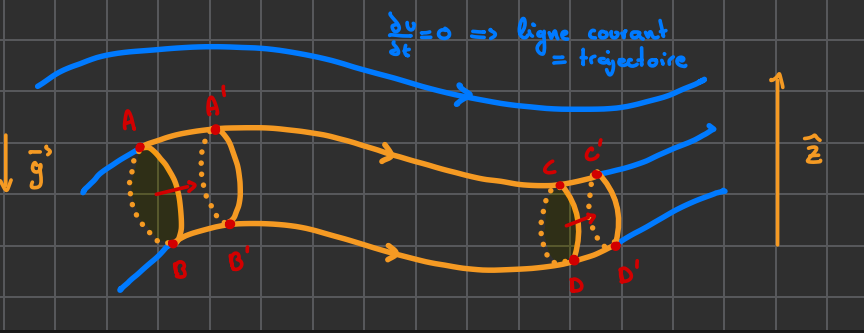
\includegraphics[width=0.8\textwidth]{images/bernoulli.png}
	\captionof{figure}{Tube de courant}
\end{minipage}
\[
\boxed{S_A u_A = S_C u_C}
\]
 on appelle ça alors la \emph{conservation du flux}. On en déduit donc que
\[
V_{ABA'B'} = S_A u_A \Delta t = S_C u_C \Delta t = V_{CDC'C'} =: \Delta V
\]
De plus puisque qu'on considère une fluide dans friction $\Delta E_{cin} + \Delta E_{pot} = \Delta W$, or
\[
\Delta E_{cin} = \frac12 \rho u_C^2 \Delta V - \frac12 \rho u_A^2 \Delta V \et \Delta E_{pot} = \rho \Delta V g z_C - \rho \Delta V g z_A
\]
De plus le travail $\Delta W$ est dû aux forces de pression agissant sur $S_A$ et $S_C$, 
\[
\Delta W = p_A S_A u_A \Delta t - p_C S_C u_C \Delta t = (p_A - p_C)\Delta V
\]
Donc on a bien
\[
\frac12 \rho u_A^2 + \rho g z_A + p_A = \frac12 \rho u_C^2 + \rho g z_C + p_C
\]

\subsection{Écoulement d'un fluide visqueux}
\subsubsection{Définition de la viscosité}
On considère une fluide \emph{incompressible} dans une situation relativement simple
\begin{figure}[H]
	\centering
	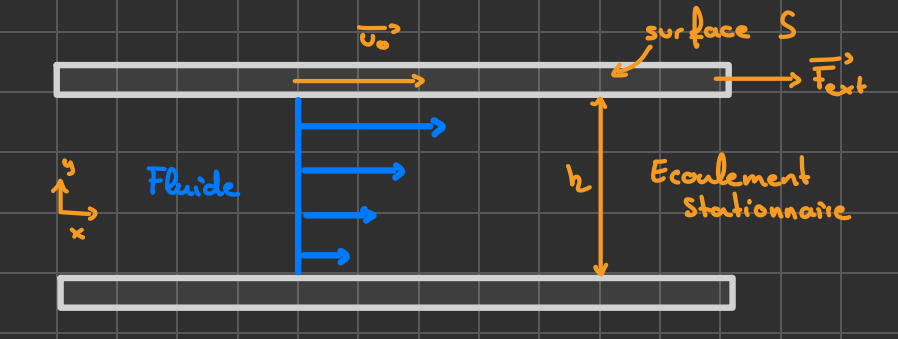
\includegraphics[width=0.35\textwidth]{images/viscosité.png}
	\caption{Écoulement stationnaire d'un fluide visqueux}
\end{figure}
Dans ce cas, l'expérience montrerai que pour déplacer la plaque supérieur à une vitesse $v_0$, il nous faudrait appliquer une force de cisaillement
 \[
 F \propto S \frac{v_0}{h}
 \]
 Ce facteur de proportionnalité est ce qu'on appelle le \emph{coefficient de viscosité dynamique} $\eta$ avec $[\eta] \mathrm N \cdot \mathrm s  \cdot \mathrm m^{-2} = \mathrm{Pa} \cdot s$. Plus généralement on a
 \[
 \boxed{F = \eta S \frac{\partial u}{\partial y}}
 \]
 On comprend alors que la viscosité permet la diffusion de la quantité de mouvement.
 
 \subsubsection{Force de viscosité et équation de Navier-Stokes incompressible}


 \begin{minipage}{0.5\textwidth}
 	\centering
 	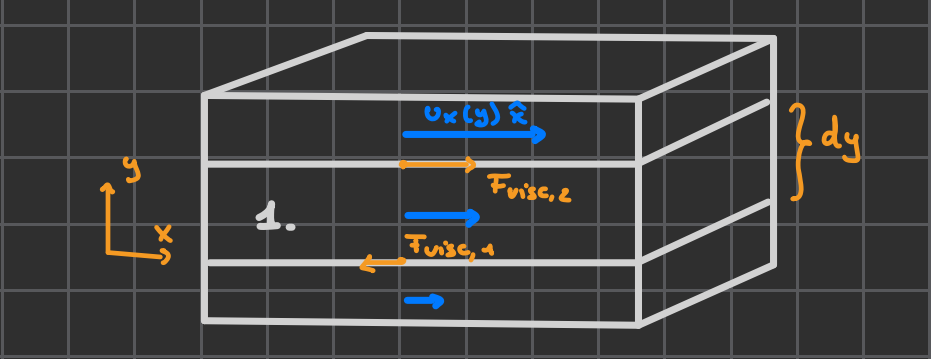
\includegraphics[width=0.8\textwidth]{images/viscosité-navier.png}
 	\captionof{figure}{uwu}
 \end{minipage}
  \hfill
 \noindent
  \begin{minipage}{0.5\textwidth}
 	On cherche à quantifier cette friction interne. Ainsi si on se place dans la situation ci-près, on a vu que la vitesse du fluide était de la forme $\bm u(\bm r, t) = u_x(y) \bm e_x$. Ainsi, la force de viscosité sur l'élément $1.$ devient
 	\begin{align*}
 		\bm F_{visc} = \bm F_{vics, 1} + \bm F_{vics, 2} &= - \eta S \frac{ \partial u_x}{\partial y}(y) \bm e_x + \eta S \frac{\partial u_x}{\partial y} (y + \mathrm d y) \bm e_x \\
 		&= \eta S \mathrm dy \frac{1}{\mathrm dy} \left( \frac{\partial u_x}{\partial y} (y + \mathrm dy) - \frac{\partial u_x}{\partial u_x}(y) \right) \bm e_x \\ &= \mathrm dV \eta \frac{\partial^2 u_x}{\partial y^2} \bm e_x
 		\end{align*}
 		 \end{minipage}
 	plus généralement, la \emph{force de viscosité} par unité de volume est donnée par 
 	\[
 	\boxed{F = \eta \Delta \bm u}
 	\]
 	où $\Delta = \nabla \cdot \nabla$. Donc pour un fluide incompressible visqueux on a deux équations
 	\[
 	\nabla \cdot \bm u = 0 \et \boxed{\rho \frac{\mathrm D \bm u}{\mathrm Dt} = \rho \bm g - \nabla p + \eta \Delta \bm u}
 	\]
 	et la condition au bord est donnée par $\bm u = 0$.

\clearpage
\section{Phénomènes ondulatoires}

\subsection{Onde traverse, longitudinale et l'équation d'onde}
L'équation de mouvement de la corde $y_0$ est solution de l'équation différentielle
\begin{equation} \label{eq: équation différentielle}
\boxed{\frac{\partial^2 y_0}{\partial t^2} = c^2 \frac{\partial^2 y_0}{\partial x^2}}
\end{equation}
avec $[c]= \mathrm m \cdot \mathrm s^{-1}$. De plus on remarque que cette équation différentielle est linéaire en $y_0$, donc si $f$ et $g$ sont deux solutions, alors $f+g$ est solution. De plus
\[
y_0(x,t) = f(x - ct) + g(x + ct)
\]
est la solution générale de cette équation.

\subsection{Ondes sinusoïdales}
On considère le cas particulier
\[
y_0(x,t) = A \cos(\omega t - kx + \varphi)
\]
où $A$ est l'\emph{amplitude}, $k$ le \emph{nombre d'onde}, $\omega$ la \emph{fréquence angulaire} et $\varphi$ le \emph{déphasage}. On vérifie facilement que $y_0$ satisfait l'équation différentielle \eqref{eq: équation différentielle}. On définit $c := \frac\omega{k}$ comme la \emph{vitesse de propagation} de l'onde et,
\begin{enumerate}
	\item Longueur d'onde : $\lambda = \frac{2\pi}k$
	\item Période : $T = \frac{2\pi}\omega$
	\item Fréquence : $\nu = \frac1T$
\end{enumerate}
on remarque dès lors que $y_0$ est solution, c'est-à-dire $c = \frac\omega{k}$, alors
\[
\boxed{\nu \lambda} = c
\]
On peut utiliser la \emph{notation} complexe pour les ondes en posant
\[
\boxed{\tilde y_0 = \tilde A e^{i(\omega t- kx)}}
\]
avec $\tilde A = A e^{i \varphi}$ et donc $y_0 = \Re(\tilde y_0)$.

\subsection{Ondes stationnaires}
On considère une \emph{onde stationnaire} qui n'est rien d'autre qu'une onde dont les extrémités $P_1$ et $P_2$ sont fixées. Ainsi la solution est de la forme,
\[
\boxed{y_0(x,t) = d \sin \left(\frac{n \pi}{l} x \right) \cos\left(\frac{c \pi}{l} nt + \varphi \right)}
\]
En effet comme l'onde est réfléchie à $P_1$ et $P_2$, on chercher alors une solution de la forme,
\[
\tilde y_0 = \tilde A_1 e^{i (\omega t - kx)} +\tilde A_2 e^{i (\omega t + kx)}
\]
En prenant en compte la condition en $P_1$ : $y_0(0,t) = 0$, ainsi
\[
\tilde y_0(0,t) = \tilde A_1e^{i \omega t} + \tilde A_2 e^{i \omega t} = 0 \implies \tilde A_1 = - \tilde A_2
\]
Ainsi on peut conclure que
\[
\tilde y_0(x,t) = \tilde A_2 2_i e^{i\omega t} \frac{(e^{i k x}- e^{-i kx})}{2i} = \underbrace{2 \tilde A_2 i e^{i \omega t}}_{d e^{i(\omega t + \varphi)}} \sin(kx)
\]
ainsi $y_0(x,t) = \Re(\tilde y_0(x,t)) = d \cos(\omega t + \varphi) \sin(kx)$. Finalement comme $y_0(p_2, t) = 0$. On définit $p_2 - p_1 =: l$, alors
\[
d \cos(\omega t \varphi) \sin{kl} = 0
\]
alors $k = \frac{n \pi}{l}$ et $\omega = \frac{cn \pi}{l}$, ainsi on a bien
\[
y_0(x,t) = d \sin \left(\frac{n \pi}{l} x \right) \cos\left(\frac{c \pi}{l} nt + \varphi \right)
\]

\subsection{Ondes en $3D$}
En 3 dimension, l'équation d'onde devient
\[
\boxed{\frac{\partial^2 y_0}{\partial t^2} = c^2 \Delta y_0}
\]
Ainsi le ondes sinusoïdales deviennent des sinusoïdales planes
\[
\tilde y_0(\bm r, t) = \tilde Ae^{i (\omega t - \bm k \cdot \bm r)}
\]
où $\bm k$ est le vecteur d'onde dont la norme décrit le nombre d'onde $k = \frac{2\pi}{\lambda}$ et donc la direction indique celle de la propagation de l'onde. Une \emph{surface équiphase} est définit comme une surface de phase $\varphi$ constante, c'est-à-dire
\[
\boxed{\omega t - \bm k \cdot \bm r = \varphi_0 = cste}
\]
on en déduit que les surfaces équiphases sont des plans, qui se déplacent à vitesse $c = \frac{\omega}{k}$ et donc la direction $\bm k$.

\subsection{Quelques conséquence du principe de superposition linéaire}
On considère deux ondes de fréquence angulaire $\omega + \Delta \omega$ et $\omega - \Delta \omega$, de vecteur d'onde $k + \Delta k$ et $k - \Delta k$, de déphasage $\varphi_1$ et $\varphi_2$, et de même amplitude. AInsi
\[
\tilde y_0 = A e^{i((\omega + \Delta \omega)t + (k + \Delta k) x + \varphi_1)} + A e^{i((\omega - \Delta \omega)t + (k - \Delta k) x + \varphi_1)}
\]
ce qui nous donne
\[
\boxed{y_0(x,t) = \Re(\tilde y_0(x,t)) = 2 A \cos \left(\frac{\varphi_1 - \varphi_2}{2} + \Delta \omega t - \Delta x \right) \cos\left( \frac{\varphi_1 + \varphi_2}{2} + \omega t - k x \right)}
\]

\clearpage
\section{Ondes dans les milieux fluides}
Si on reprend les équations de continuité, d'Euler et d'état en négligeant la gravité et partant du principe que l'on a un gaz parfait, alors les équation deviennent
\[
\frac{\partial \rho}{\partial t} + \nabla \cdot (\rho \bm u) = 0, \quad \rho \left( \frac{\partial \bm u}{\partial t} + (\bm u \cdot \nabla ) \bm u \right) = - \nabla p, \quad \frac{\mathrm D}{\mathrm Dt} (p \rho^{-\gamma}) = 0
\]
En équilibre $\rho = \rho_0 = cste$, $\bm u = 0$ et $p = p_0 = cste$. On y ajoute alors des \emph{petites perturbations} $\rho_1, p_1, \bm u_1$, alors on obtient que les paramètres décrivant le fluides sont
\[
\rho = \rho_0 + \rho_1, \quad \bm u = \bm u_1, \quad p = p_0 + p_1
\]
Ainsi en linéarisant l'équation de continuité on trouve
\[
\frac{\partial(\rho_0 + \rho_1)}{\partial t} + \nabla (\rho_0 \bm u_1 + \rho_1 \bm u_1) = 0 \implies \boxed{\frac{\partial \rho_1}{\partial t} + \rho_0 \nabla \cdot \bm u = 0 }
\]
l'équation d'Euler devient
\[
(\rho_0 + \rho_1) \left( \frac{\partial \bm u_1}{\partial t} + (u_1 \cdot \nabla) \bm u_1 \right) = - \nabla (p_0 + p_1) \implies \boxed{\rho_0 \frac{\bm u_1}{\partial t} = - \nabla p_1}
\]
et finalement l'équation d'état devient
\[
\left(\frac{\partial }{\partial t} + (\bm u_1 \nabla)\right) \left( \frac{p_0 + p_1}{(\rho_0 + \rho_1)^\gamma}\right) = 0 \implies \boxed{\frac{\partial p_1}{\partial t} - \frac{\gamma p_0}{\rho_0} \frac{\partial p_1}{\partial t} = 0}
\]
On cherche alors des solutions de la forme
\[
\rho_1(\bm r, t) = \tilde \rho_1 e^{i(\omega t - \bm k \cdot \bm r)}, \quad \bm u_1(\bm r, t) = \bm{\tilde u}_1 e^{i(\omega t - \bm k \cdot \bm r)}, \quad p_1(\bm r, t) = \tilde p_1 e^{i(\omega t - \bm k \cdot \bm r)}
\]
En utilisant le fait que si $f$ est solution complexe d'une équation diffénrentielle, alors $\Re f$ l'est aussi, on trouve que
\[
\tilde \rho_1 = \frac{\rho_0}{\gamma p_0} \tilde p_1 \et \bm{\tilde u}_1 = \frac{\bm k}{\omega \rho_0} \tilde p_1
\]
ainsi on peut en déduire qu'on une onde longitudinale le long de $\bm k$, en choisissant $\bm k = k \bm e_z$ et $\bm{\tilde u}_1 = \tilde u_1 \bm e_z$, on obtient
\[
\boxed{\rho_1(\bm r,t) = \frac{\rho_0}{\gamma p_0} \tilde p_1 e^{i(\omega t - kz)}}, \quad \boxed{\bm{\tilde u}_1= \frac{\bm k}{\omega \rho_0}\tilde p_1 e^{i(\omega t -kz)}}, \quad \boxed{p_1(\bm r,t) = \tilde p_1 e^{i (\omega t - kz)}}	
\]
De plus on sait que $c = \frac{\omega}{k} = \sqrt{\gamma \frac{p_0}{\rho_0}}$ mais d'après la loi des gaz parfait $pV = nRT$, on obtient $\frac{p}{\rho} = \frac{RT}{m}$ et donc
\[
\boxed{c = \sqrt{\gamma\frac{RT}{m}}}
\]

\clearpage
\section{Électromagnétisme}
\subsection{Loi de Coulomb}
Si on considère deux \emph{charges ponctuelles} $q_1$ et $q_2$. Alors la force exercée par $q_1$ sur $q_2$ est
\[
\boxed{\bm F_{1 \to 2} = \frac{1}{4 \pi \varepsilon_0} \frac{q_1 q_2}{\norme{\bm r_{12}}^2} \frac{\bm r_{12}}{\norme{\bm r_{12}}}}
\]
où $\bm r_{12} = \bm r_2 - \bm r_1$ et $\varepsilon_0 = 8.85 \cdot 10^{-12} ~\mathrm F \cdot \mathrm m^{-1}$. De plus on remarque que $\bm F_{1 \to 2} = - \bm F_{2 \to 1}$. SI on considère $n$ \emph{charges ponctuelles} $q_i$ à $\bm r_i$, alors la force exercée sur une charge $q$ à $\bm r$ est 
\[
\boxed{\bm F_{res} = \sum_{i=1}^n \bm F_{i \to q}}
\]
ce qu'on appelle le \emph{principe de superposition}

\subsection{Champ électrique}
D'après la loi de coulomb, on a vu que
	\[
	\bm F_{i \to q} = {\color{violet} \frac{1}{4 \pi \varepsilon_0} \frac{q_i}{\norme{\bm r - \bm r_i}} \frac{\bm r - \bm r_i}{\norme{\bm r - \bm r_i}}} \cdot q
	\]
	où la partie en \textcolor{violet}{violet} est indépendante de la charge $q$, on appelle ce champ vectorielle le \emph{champ électrique} $\bm E$ générée par $q_i$. Plus généralement, par le principe de superposition on définit le champ électrique $\bm E$ en $\bm r$ générée par $n$ charges $q_i$ en $\bm r_i$ comme
	\[
	\boxed{\bm E (\bm r) = \sum_{i=1}^n \frac{1}{4 \pi \varepsilon_0}  \frac{q_i}{\norme{\bm r- \bm r_i}^2} \frac{\bm r - \bm r_i}{\norme{\bm r - \bm r_i}}}
	\]
	On a donc $\bm F_{res}(\bm r) = \bm E(\bm r) q$, ainsi le champ $\bm E$ est colinéaire à la direction de la force ressentie au point $\bm r$.
	
	Supposons qu'on ait une distribution de charge quelconque, on définit alors la \emph{densité de charge} et la \emph{densité de charge de surface} comme
	\[
	\boxed{\rho_{el} (\bm r) = \lim_{\Delta V \to \mathrm d V} \frac{\Delta q}{\Delta V}} \et  \boxed{\sigma_{el} (\bm r) = \lim_{\Delta S \to \mathrm d S} \frac{\Delta q}{\Delta S}}
	\]
	donc la définition de champ électrique $\bm E$ devient
	\[
	\boxed{\bm E (\bm r) = \frac{1}{4 \pi \varepsilon_0} \iiint_V \rho_{el}(\bm R) \frac{\bm r - \bm R}{\norme{\bm r  - \bm R}^3} \mathrm dV} \et \boxed{\bm E(\bm r) = \frac{1}{4 \pi \varepsilon_0} \iint_S \sigma_{el} (\bm R) \frac{ (\bm r- \bm R)}{\norme{\bm r- \bm R}^3} \mathrm d S }
	\]
	Les lignes de champs électriques sont tangentielle à $\bm E$ en chaque point point de l'espace. Elle sont orienté dans le direction de $\bm E$.
	
\subsection{Loi de Gauss}
Le \emph{flux} d'un champ électrique à travers la surface $S = \partial V$ est égale à la somme des charges électrique dans le volume $V$, divisé par la permittivité du vide, c'est-à-dire
\[
\boxed{\Phi = \iint_S \bm E \cdot \mathrm d \bm S = \frac{1}{\varepsilon_0} \iiint_V \rho_{el} \mathrm dV}
\]
on bien sous forme différentielle
\[
\boxed{\nabla \cdot \bm E = \frac{\rho_{el}}{\varepsilon_0}}
\]
En effet si on considère un charge ponctuelle $q$ au centre d'une surface $S$ sphérique de rayon $r$, on remarque que comme $E // \mathrm d\bm S$, alors
\[
\int_S \bm E \cdot \mathrm d \bm S = \int_S \norme{\bm E} \cdot \mathrm d \bm S = \frac{1}{4 \pi \varepsilon_0} \frac{q}{r^2} 4\pi r^2 = \frac{q}{\varepsilon_0}
\]
Ainsi, la loi de Gauss est satisfaite dans ce cas. 


\noindent
\begin{minipage}{0.66\textwidth}
On considère maintenant le cas où une charge $q$ est entouré d'une surface fermée $S$ quelconque. On a donc les relations suivantes
\[
\Phi_{\mathrm d S'} = E' \mathrm d S' \et \phi_{\mathrm d \bm S} = E \mathrm dS \cos\theta
\]
Or
\[
E = E' \frac{r'^2}{r'2} \et \mathrm d  S = \mathrm d S' \frac{r^2}{r'^2} \frac{1}{cos\theta}
\]
donc
\[
\phi_{\mathrm d \bm S} \cos \theta= E \mathrm dS \cos\theta = E' \frac{r'^2}{r'2} d S' \frac{r^2}{r'^2} \frac{1}{cos\theta} \cos \theta = E' \mathrm dS' = \Phi_{\mathrm d S'}
\]

\end{minipage}
\hfill
\begin{minipage}{0.3\textwidth}
	\centering
	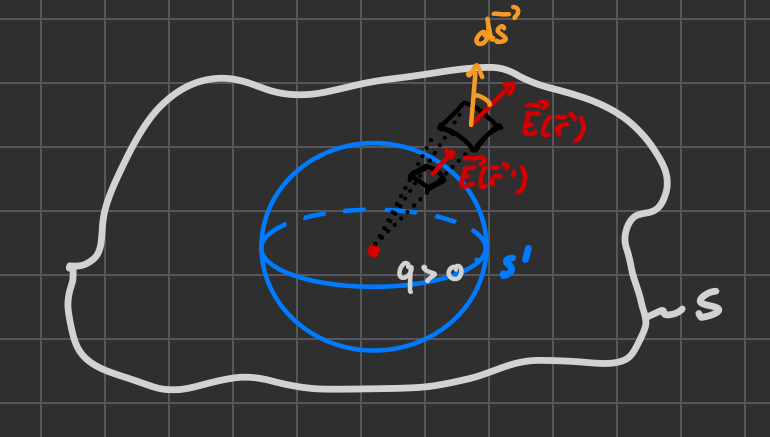
\includegraphics[width=0.8\textwidth]{images/loi-de-gauss.png}
	\captionof{figure}{Charge $q$ entouré d'une surface fermée $S$.}
\end{minipage}
Ceci étant valable pour n'importe quel éléments de surface $\mathrm d S$ donc
\[
\Phi = \iint_S \bm E \cdot \mathrm d \bm S = \iint_{S'} \bm  E' \cdot \mathrm d \bm S' = \frac{q}{\varepsilon_0}
\]

\begin{minipage}{0.3\textwidth}
	\centering
	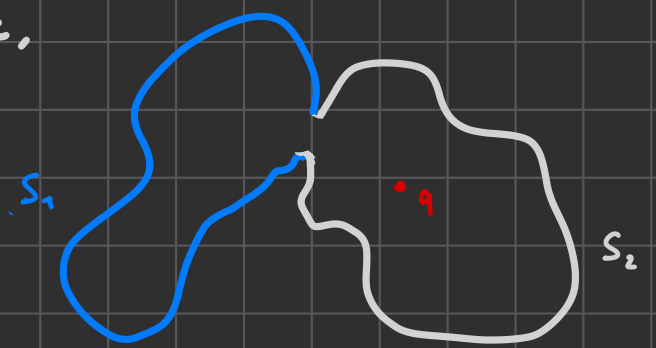
\includegraphics[width=0.8\textwidth]{images/lacet-uwu.png}
	\captionof{figure}{Surface {\color{blue} $S$} à l'éxtérieur de la charge $q$.}
\end{minipage}
\hfill
\begin{minipage}{0.6\textwidth}
	On considère le dernier cas où on a un charge ponctuelle $q$ à l'extérieur d'une surface $S$ arbitraire comme ci-près. Ainsi par le point 2.
	\begin{align*}
	\frac{q}{\varepsilon_0} &= \iint_{S_1 + S_2}\bm  E \cdot \mathrm d \bm S  \\
	&= \iint_{S_1} \bm E \cdot \mathrm d \bm S + \iint_{S_2} \bm E \cdot \mathrm d \bm S \longrightarrow \iint_S \bm E \cdot \mathrm d \bm S + \frac{q}{\varepsilon_0}
	\end{align*}
	Ainsi lorsque la charge est à l'extérieur, on trouve bien
	\[
	\iint_S \bm E \cdot \mathrm d \bm S = 0
	\]
\end{minipage}

\subsection{Le potentiel électrostatique}
En électrostatique, on peut définir un champ scalaire $\phi(\bm r)$ tel que
\[
\boxed{\bm E = - \nabla \phi}
\]
On appelle $\phi$ le \emph{potentielle électrostatique}. Par exemple, pour une charge ponctuelle $q_1$ à $\bm r_1$ on a
\[
\phi(\bm r) = \frac{1}{4 \pi \varepsilon_0} \frac{q_1}{\norme{\bm r - \bm r_1}} + cste
\]
qu'on vérifie facilement en appliquant le gradient. Pour une distribution de charge arbitraire on a
\[
\boxed{\phi(\bm r) = \frac{1}{4 \pi \varepsilon} \iiint_V \frac{\rho_{el} (\bm R)}{\norme{\bm r - \bm R}} \mathrm dV + cste}
\]
On remarque alors que $\phi$ doit avoir une unité $[\phi] = V $. Puisque que le rotationel  du gradient d'un champ scalaire est nécessairement nul, alors
\[
\boxed{\nabla \times \bm E = \bm 0}
\]
Le travail pour déplacer une charge $q$ dans un champ $\bm E$ de $A$ é $B$ ne dépend pas du champin suivit et vaut
\[
\boxed{W = q(\phi(A) - \phi(B))}
\]
\begin{minipage}{0.7\textwidth}
	En effet, soit $\gamma$ le chemin paramétré par $\bm l( s)$, alors
	\begin{align*}
	W_{\gamma} = \int_{\gamma} \bm F \cdot \mathrm \bm l = - \int_\gamma q \bm E \cdot \mathrm d \bm l 
	&= \int_\gamma q \nabla \phi \cdot \mathrm d \bm l \\&= \int_0^1 q \nabla \phi( \bm l(s)) \cdot \frac{\mathrm d \bm l}{\mathrm d s} \mathrm d s = q \phi(\bm l(s)) \big|_0^1 = q(\phi(B) - \phi(A))
	\end{align*}
\end{minipage}
\hfill
\begin{minipage}{0.2\textwidth}
	\centering
	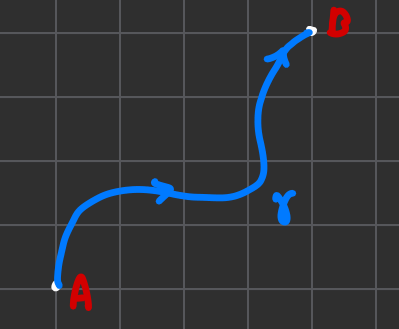
\includegraphics[width=0.8\textwidth]{images/aàb.png}
	\captionof*{figure}{Chemin $\gamma$}
\end{minipage}
Il en suit que le travail pour déplacer une charge $q$ le long d'une courbe fermé est nul. Ainsi on en déduit que $\bm F = q \bm E$ est une force conservatrice. 

Pour une charge ponctuelle de charge $q$ et masse $m$, et pour un champ gravitationnel $\bm g = - g \bm e_z$, l'énergie mécanique plus générale est désormais
\[
\boxed{E_{tot} = \frac12 m \norme{\bm u}^2 + q \phi(\bm x) + mg z}
\]
De plus la différence de potentielle électrique par unité de charge d'une particule entre les positions $A$ et $A$ est donnée par
\[
\boxed{\phi(B) - \phi(A) = - \int_{A \to B} \bm E \cdot \mathrm d \bm l}
\]
Ce qui est une méthode souvent utile pour calculer le potentielle électrique directement à partir de $\bm E$.

Finalement, une dernière remarque sur $\phi$, comme $\bm E = - \nabla \phi$, les lignes de champ électrique sont partout perpendiculaire aux surfaces équipotentielles de par la nature du gradient.

\subsection{Le rôle des conducteurs en électrostatique}
\subsubsection{Propriétés de bases}
\begin{minipage}{0.6\textwidth}
En électrostatique, il n'y a \textbf{PAS} de courant dans un conducteur et donc
\begin{enumerate}
	\item $\bm E = 0$ à l'intérieur d'un conducteur $\implies \phi = cste$ dans le conducteur.
	\item $\nabla \cdot E = 0 \implies \rho_{el} = 0$ par le loi de Gauss
	\item Puisque $E$ est perpendiculaire au isosurface alors $E$ est perpendiculaire à la surface extérieure du conducteur car $\phi = cste$.
	\item Des charges peuvent se trouver uniquement à la surface du conducteur, avec $\norme{\bm E} = \frac{\sigma_{el}}{\varepsilon_0}$.
\end{enumerate}
\end{minipage}
\hfill
\begin{minipage}{0.4\textwidth}
	\centering
	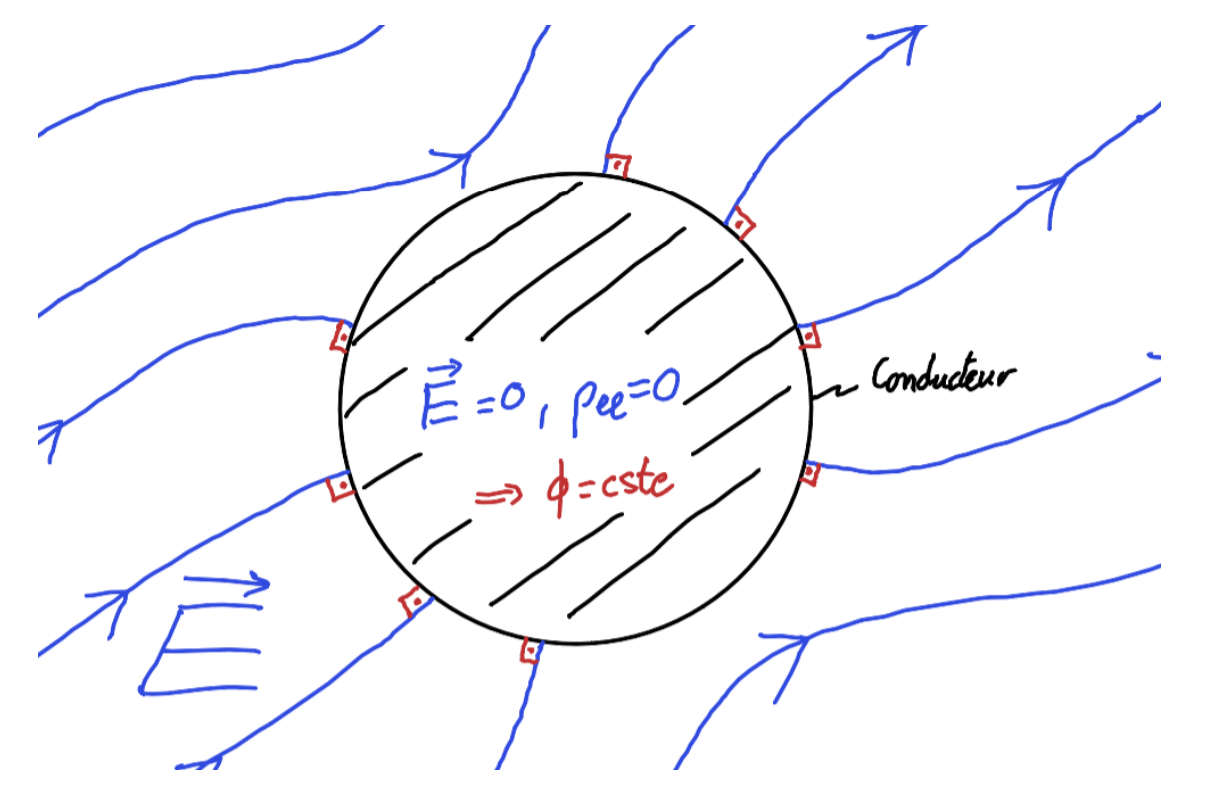
\includegraphics[width=0.9\textwidth]{images/conducteur.png}
	\captionof*{figure}{Chemin $\gamma$}
\end{minipage}

\subsubsection{Densité de charge surfacique par influence électrostatique}
On considère un champ électrique $\bm E$ uniforme et une plaque conductrice non-chargée, avec $\bm E$ perpendiculaire à la plaque comme ci-dessous
\begin{figure}[H]
	\centering
	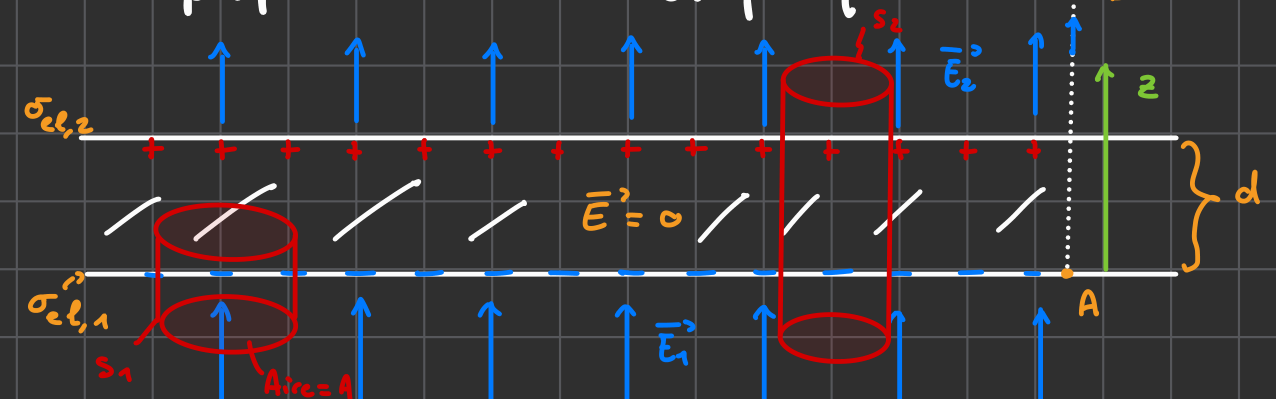
\includegraphics[width=0.6\textwidth]{images/densité-de-charge.png}
	\caption{plaque conductrice non-chargée.}
\end{figure}
Si on applique la loi de Gauss à $S_1$, on obtient
\[
\iint_S \bm E_1 \cdot \mathrm d \bm S = \frac{1}{\varepsilon_0} \iiint_V \rho_{el} \mathrm d V \implies -E_1 A = \frac{\sigma_{el,1} A}{\varepsilon_0}
\]
ainsi $\sigma_{el,1} = - \varepsilon_0 E_1$. Comme le conducteur est non-chargé, alors $\sigma_{el,2} = - \sigma_{el,1}$. Donc en appliquant Gauss sur $S_2$, on trouve
\[
A E_2 - A E_1 = \frac{\sigma_{el,1} + \sigma_{el,2}}{\sigma_0} = 0
\]
Ce qui implique donc que $E_1 = E_2 = E_0$. Comme $\bm E \| \bm $ alors $\phi(x,y,z) = \phi(z)$. Choisissons $B$ à hauteur $z$ et $A$ à hauteur $0$ avec $\phi(z = 0) = 0$. Donc
\[
\phi(z) = \phi(z) - \phi(0) = -\int_0^z \bm E \cdot \mathrm d \bm l = - \int_0^z \bm E \cdot \bm e_z ~\mathrm d z' = -\int_0^z E_z(z') \mathrm d z'
\]
Ainsi si $z < 0$, on a
\[
\phi(z) = -\int_0^z E_z(z') \mathrm d z' = \int_z^0 E_z(z') \mathrm d z' = E_0 \int_z^0 \mathrm d z' = -z E_0
\]
Si $0 < z < d$ alors
\[
\phi(z) z' = -\int_0^z E_z(z') \mathrm d z' = 0
\]
Et finalement si $z > d$, alors
\[
\phi(z) = -\int_d^z E_0 \mathrm d z' = (d-z) E_0
\]

\subsubsection{Effet de pointe}
Autour des points d'un conducteur le champ électrique $\bm E$ peut être très élevés 
\begin{figure}[H]
	\centering
	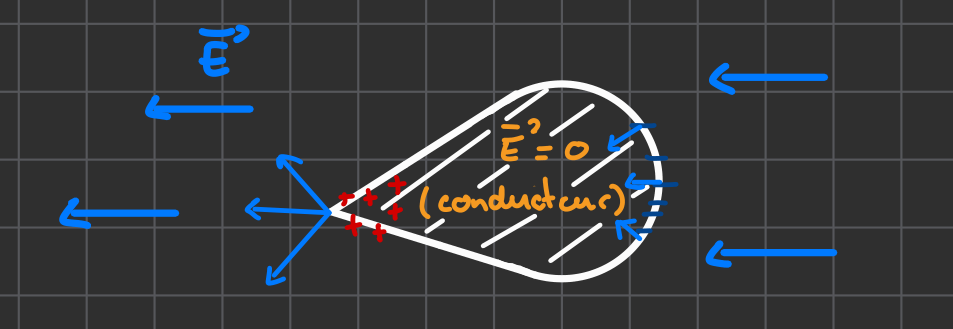
\includegraphics[width=0.6\textwidth]{images/effet-pointe.png}
	\caption{Effet de pointe}
\end{figure}
Donc si on considère un conducteur mise à haut tension, l'air est alors fortement ionisé autour des pointes du conducteur. Et donc selon la forme de l'objet, les décharges seront plus ou moins continues.

\subsubsection{Traitement générale, équation de Laplace et de Poison}
En principe, on a la loi de Gauss
\[
\nabla \cdot \bm E = \frac{\rho_{el}}{\varepsilon_0}
\]
qui permet de calculer $E$ à partir de $\rho_{el}$. Or en pratique souvent $\rho_{el}$ n'est pas connu partout. Si on considère la cas particulier où on a des conducteurs placés à des potentielles différents.
\begin{figure}[H]
	\centering
	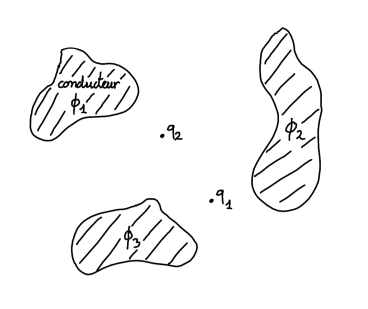
\includegraphics[width=0.3\textwidth]{images/équation-laplace}
\end{figure}
On connait alors le potentiel à la surface de chaque conducteur, mais pas $\sigma_{el}$. Par contre si l'on sait que $\rho_{el} = 0$ à l'extérieur des conducteurs (donc dans le cas où $q_1$ et $q_2$ sont absent), alors $\nabla \cdot \bm E = 0$. Comme $\bm E$ dérive d'un potentiel, alors on l'\emph{équationde Laplace}
\[
- \nabla \cdot \bm E = \boxed{\Delta \phi = 0}
\]
Et si $\rho_{el} \neq 0$ entre les conducteur, alors on l'\emph{équation de poisson}
\[
\boxed{\Delta \phi = - \frac{\rho_{el}}{\varepsilon_0}}
\]
Ainsi il suffit de résoudre l'équation de Laplace (ou de Poisson) en dehors des conducteurs muni des conditions limites (valeurs de $\phi$ sur les conducteurs et à l'infini si le domaine est non borné).

\subsection{Capacité et condensateur}

\subsubsection{Définition de la capacité}
\noindent
\begin{minipage}{0.6\textwidth}
	On considère deux conducteurs initialement non-chargé ($\phi_A = \phi_B = 0$), puis une charge $q_-$ est enlevé de $A$ et place sur $B$. Ainsi on remarque que
	\[
	\phi_A - \phi_B = - \int_{P_A}^{P_B} \bm E \cdot \mathrm d \bm l > 0
	\]
	De plus on a que $\bm E$ est proportionnel à $q$ et donc $\phi_A - \phi_B$ aussi, ainsi
	\[
	\frac{q}{\phi_A - \phi_B} = cste := C
	\]
\end{minipage}
\hfill
\begin{minipage}{0.4\textwidth}
	\centering
	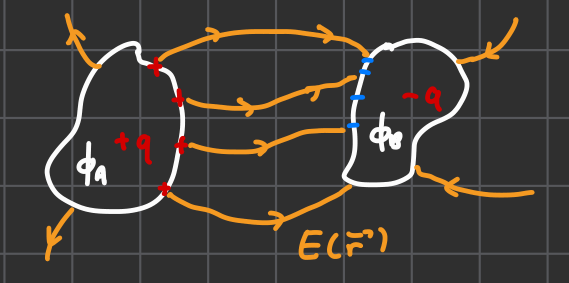
\includegraphics[width=0.8\textwidth]{images/capactié.png}
	\captionof{figure}{définition de la capacité}
\end{minipage}
Souvent on préfère écrire $U = \phi_A - \phi_B$. donc la relation devient
\[
\boxed{C = \frac{q}{U}}
\]
avec $[C] = \unit{c.V^{-1}}$. On appelle cette constante $C$ la \emph{capacité} entres les deux conducteurs. Su les conducteurs sont entourés de vide, $C$ ne dépend que de la géométrie des condensateurs.

\subsubsection{Le condensateur}
Un \emph{condensateur} est un système de deux conducteurs avec des charges $\pm q$. Généralement, la géométrique est choisie pour maximiser le rapport capacité et volume
\[
\boxed{Q = CU}
\]
Ainsi si on considère un condensateur cylindrique \\ \\
\begin{minipage}{0.4\textwidth}
	\centering
	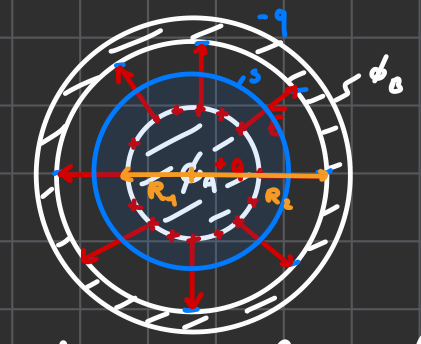
\includegraphics[width=0.8\textwidth]{images/condensateur-cylindrique.png}
	\captionof{figure}{définition de la capacité}
\end{minipage}
\hfill
\begin{minipage}{0.6\textwidth}
	On suppose que $l \gg R_2 - R_1$, on peut donc négliger les effets de bords, donc par Gauss
	\[
	\iint_S \bm E \cdot \mathrm d \bm S = \frac{1}{\varepsilon_0} \iiint_V \rho_{el} \mathrm dV \implies 2 \pi rl \bm E(r) = \frac{q}{\varepsilon_0}
	\]
	Donc $\bm E (r) = \frac{q}{2 \pi  rl \varepsilon_0}$. De plus
	\[
	\phi_A - \phi_B = \int_{R_1}^{R_2} \bm E \cdot \mathrm d \bm l = - \int_{R_1}^{R_2}  E(r) \bm e_r \cdot \bm e_r \mathrm dr = -\int_{R_1}^{R_2} E(r) \mathrm dr
	\]
\end{minipage}
Donc par ce qui précède on en déduit que
\[
\phi_A - \phi_B = - \frac{q}{2 \pi \varepsilon_0 l} \int_{R_1}^{R_2} \frac{1}{r} \mathrm d r = - \frac{q}{2 \pi \varepsilon_0 l} \log \left(\frac{R_2}{R_1} \right)
\]
on peut donc en conclure que
\[
C = \frac{q}{\phi_B - \phi_A} = \frac{2 \pi \varepsilon_0 l}{\log{R_2} - \log{R_1}}
\]
\subsubsection{Énergie stockée dans un condensateur et densité d'énergie électrique}
Le travail pour déplacer une charge $- \mathrm dq$ du conducteur $A$ au conducteur $B$ est
\[
\mathrm d W = (\phi_B - \phi_A)(- \mathrm dq) =(\phi_A -\phi_B) \mathrm dq = U \mathrm d q = \frac{q}{C} \mathrm dq
\]
Ainsi le travail pour \emph{charger} le condensateur à la charge $q$ est 
\[
W = \int_0^q \mathrm d W = \int_0^q \frac{1}{C} \tilde q \mathrm d \tilde q = \frac{1}{2C} q^2 = \frac{1}{2} C U^2
\]
par exemple, pour un condensateur plan
\[
W =  \frac12 CU^2  = \frac12 \frac{\varepsilon_0 S_c}{d} E^2 d^2 = \frac12 \varepsilon_0 E^2 S_c d
\]
où $S_c d$ correspond au volume entre les plaques. On peut alors interpréter ce résultat en disant que le travail $W$ est stocké dans le champ $\bm E$ sous forme de \emph{densité d'énergie électrique} $e_E = \frac{1}{2} \varepsilon_0 E^2$. De manière générale
\[
\boxed{e_E = \frac12 \varepsilon_0 E^2}
\]
exprime la densité d'énergie électrique, pour une configuration arbitraire.

\subsection{Capacité avec un diélectrique}

Un \emph{diélectrique} est un isolant, c'est-à-dire qu'il de contient pas de porteurs de charge libre. Par expérience, on remarque que si on remplace le vide dans un condensateur par un diélectrique, alors $U$ diminue donc $C$ \textbf{augmente}. En effet sa \emph{densité d'énergie électrique avec diélectrique} est désormais donné par
\[
\boxed{e_E =  \frac12 \varepsilon_0 \varepsilon_r E^2}
\]
où $\varepsilon_r$ est la \emph{permittivité relative} de l'isolant. De plus si $C$ est la capacité d'un condensateur sans diélectrique, alors $\varepsilon_r C$ est sa capacité avec diélectrique.

\clearpage

\section{circuit électrique}
En présence d'une \emph{présence électromotrice}, c'est-à-dire une grandeur qui caractérise un dispositif capable de fournir de l'énergie aux charges et d'imposer une différence de potentiel entre deux bornes. Un champ électrique peut alors être maintenue dans un conducteur, ce qui met en mouvement les porteurs de charges et produit un courant.

\subsection{Définition du courant}
On définit le \emph{courant} comme le \emph{flux de charge} par unité de temps à travers une surface $S$. En particulier
\[
\boxed{I = \dot q}
\]
avec $[I] = \unit{A}$. De plus on définit la \emph{densité de courant} comme
\[
\bm j (\bm r, t) = \rho_{el}^{\mathrm{mobile}} (\bm r, t) \bm u(\bm u, t) = q n(\bm r, t) \bm u(\bm r, t)
\]
avec $[j] = \unit{A.m^{-2}}$. $\bm j$ correspond au courant traversant une surface par unité de surface, avec $\mathrm \bm I = \bm j \cdot \mathrm d \bm S$. On peut alors exprimer le courant en fonction de $\bm j$,
\[
I(t) = \iint_S \bm j \cdot \mathrm d \bm S
\]

\subsection{La résistance, la loi d'Ohm et l'effet Joule}
La résistance d'un objet caractérise le courant qui le traverse en fonction de la tension appliquée
\[
\boxed{R = \frac{U}I}
\]
La résistance ce mesure en Ohms : $[R] = \unit{VA^{-1}} = \unit{\Omega}$. Dans certain cas, le courant est proportionnel à la tension. Donc la résistance en indépendante de $U$, on parle alors de la loi d'Ohm,
\[
\boxed{R = \frac{U}{I} = cste}
\]
De manière générale, la loi d'Ohm s'écrit
\[
\bm j = \sigma_c \bm E = \frac{1}{\rho_c} \bm E
\]
avec $\sigma_c$ est la \emph{conductibilité électrique} mesuré en $\unit{\Omega^{-1}.m^{-1}}$ et $\rho_c$ est la \emph{résistivité électrique} mesuré en $\unit{\Omega.m}$. Ces constantes dépendent du matériel. On remarque que l'on peut dériver $U = RI$ à partir de $\bm j = \sigma_c E$, en effet
\[
U = \phi_A - \phi_B = El = \frac{j}{\sigma_c} l = \frac{jS}{\sigma_c S} l = \frac{l}{\sigma_c S} I = R I
\]
Donc $U = RI$ avec
\[
\boxed{R = \frac{l}{\sigma_c S}}
\]
Tout ce transfort de charge viens cependant un coût. Si une charge $q$ se déplace de $A$ à $B$, son énergie potentielle est réduite de $q(\phi_A - \phi_B)$. Dans une résistance, cette énergie est transformée sous forme de chaleur. C'est l'\emph{effet Joule}. La puissance associée est donc
\[
P = \frac{\mathrm dW}{\mathrm dt} = \frac{\mathrm d q \cdot(\phi_A - \phi_B)}{\mathrm dt} = (\phi_A - \phi_B) \frac{\mathrm q}{\mathrm dt} = UI
\]
Cette puissance est fourni par l'appareil à f.é.m.

\subsection{Conservation de charge, équation de continuité}
\begin{minipage}{0.6\textwidth}
Par ce qui précède on sait que
\[
\frac{\mathrm d}{\mathrm dt} \iiint_V \rho_{el} \mathrm d V = - \iint_S \bm j \cdot \mathrm d \bm S
\]
ainsi par le théorème de la divergence on en déduit que
\[
\iiint_V \frac{\partial \rho_el}{\partial t} \mathrm d V = - \iiint_V \nabla \cdot \bm j \mathrm d V
\]
Or comme cette égalité est vrai pour tout volume $V$ on en déduit l'\emph{équation de continuité}
\[
\boxed{\frac{\partial \rho_{el}}{\partial t} + \nabla \cdot \bm j = 0}
\]
\end{minipage}
\hfill
\begin{minipage}{0.4\textwidth}
	\centering
	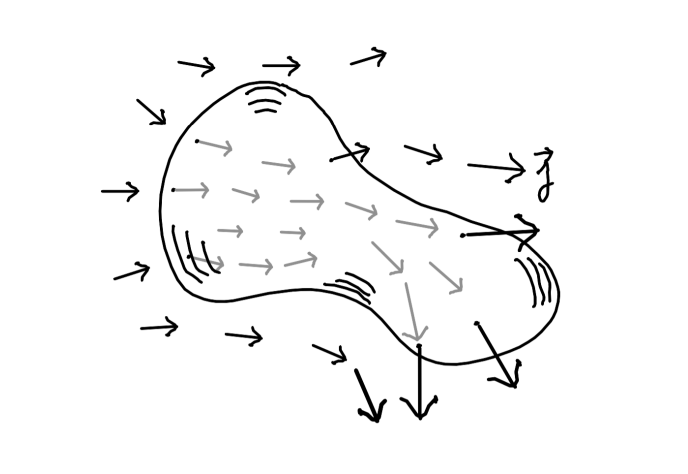
\includegraphics[width=0.8\textwidth]{images/équation-continuité.png}
	\captionof*{figure}{Volume $V$ fixé avec une surface $S$}
\end{minipage}

\subsection{Circuits électriques et lois de Kirchhoff}
On considère un circuit composée d'une \emph{source de tension continue} (appareil à FEM), de \emph{résistance}, de \emph{capacité} et d'un fil (un élément de résitance négligeable, ainsi la tension est constante le long de celui ci)
\begin{figure}[H]
	\centering 
	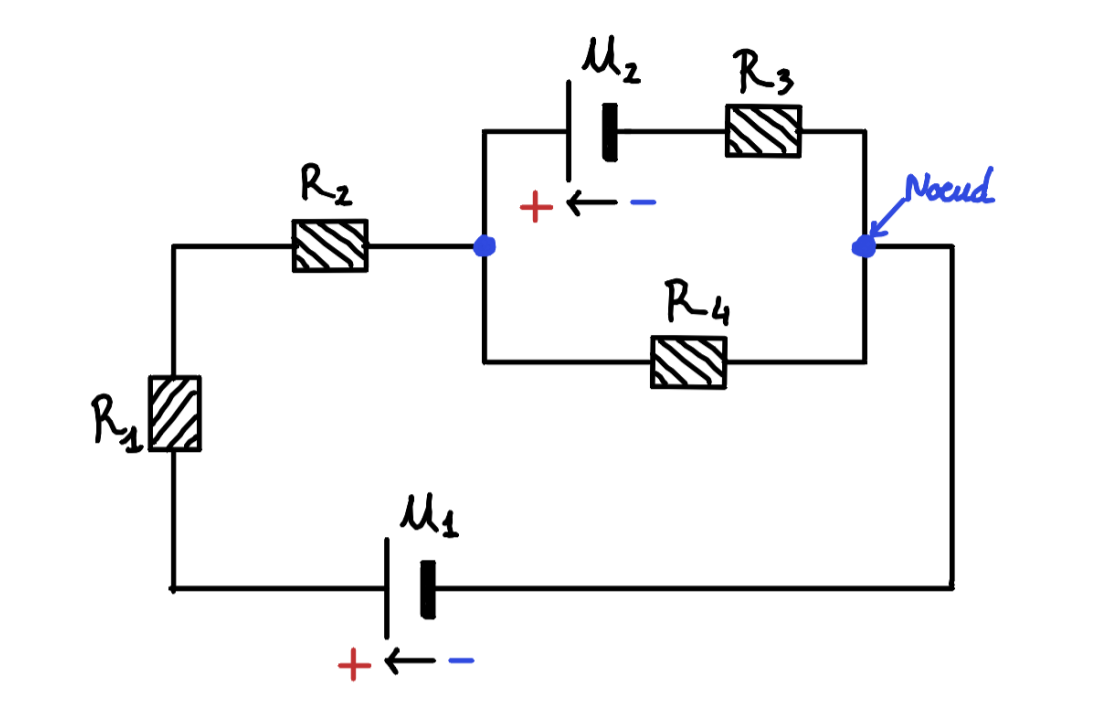
\includegraphics[width=0.4\textwidth]{images/circuit-electrique.png}
	\caption{exemple d'un circuit électrique}
\end{figure}
On a alors deux loi permettant de trouver la valeurs de différents composants du circuits
\subsubsection*{Loi des n\oe uds}
La somme de touts les courants qui arrivent au nœud d'un circuit est égale à la somme de tous le courant qui le quittent. En effet il s'agit d'une conséquence de l'équation de continuité
\[
\frac{\partial \rho_el}{\partial t} + \nabla \cdot \bm j = 0
\]
et de l'hypothèse d'un régime stationnaire $(\frac{\partial \rho}{\partial t} = 0)$. On obtient alors que $\nabla \cdot \bm j = 0$, cette dernière équation signifie que le flux de courant est conservé : il y a donc autant de courant qui entre dans le n \oe uds que de courant qui en sot.

\subsubsection*{Loi des mailles}
La somme algébriques des variations de potentiel le long de toutes mailles fermées d'un circuit en nulle. En effet, dans le cadre de l'électrostatique, ou lorsque les variations temporlles sont négligeable, on a
\[
\oint_\gamma \bm E \cdot \mathrm d \bm l = 0
\]
En supposant en outre que le potentiel ne varie par le long d'un fil, on obtient la loi des mailles de Kirchoff.

Ainsi, on définit un sens de courant quelconque sur le circuit en on résous un système d'équation provenant des lois de n\oe uds et des mailles.
\begin{figure}[H]
	\centering
	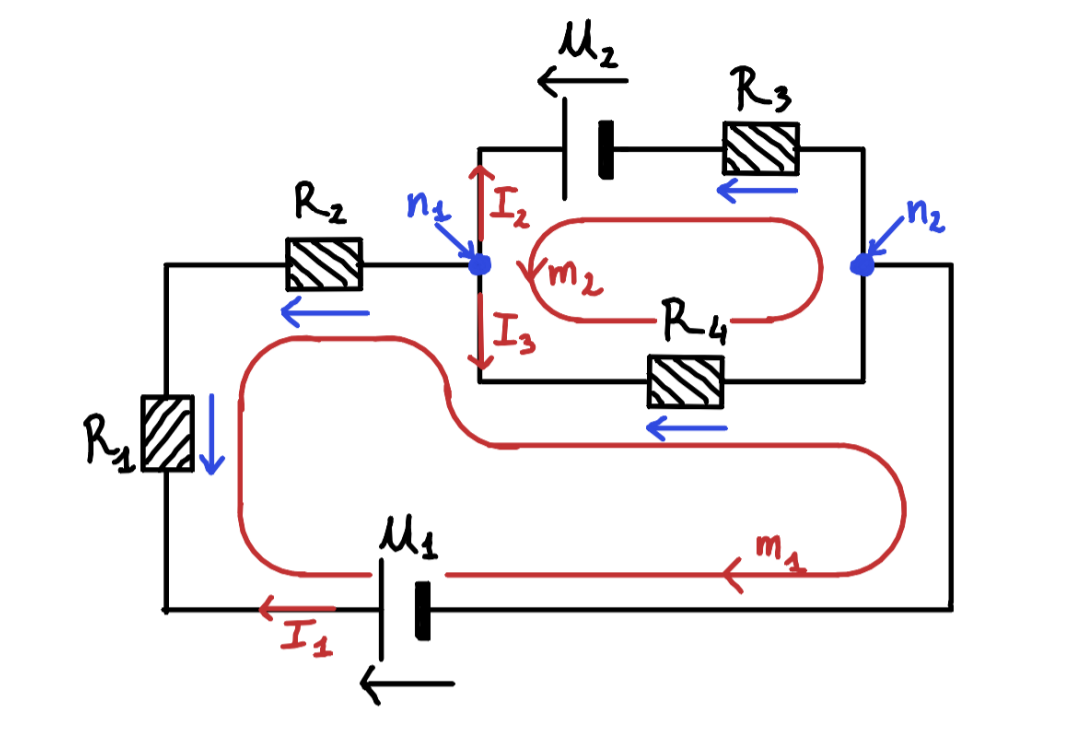
\includegraphics[width=0.4\textwidth]{images/kirchhoff.png} 
	\caption{Loi de Kirchhoff}
\end{figure}

Ainsi par kirchhoff on peut en déduire que si on a deux résistance en série alors 
\[
R_{\mathrm{equiv}} = R_1 + R_2
\]
Tandis que les deux résitances sont en parallèle on a
\[
R_{\mathrm{equiv}} = \left(\frac{1}{R_1} + \frac{1}{R_2} \right)^{-1}
\]
\clearpage
\section{Magnétostatique}

\subsection{Définition du champ magnétique et force de Lorentz}
 Un champ magnétique $\bm B$ est généré par un aimant ou un courant, et exerce une force sur un aimant ou un courant. La direction de $\bm B$ est défini üar l'orientation d'une boussole. Des expériences montrent que la force exercée sur une charge $q$ de vitesse $\bm v$ est 
 \begin{enumerate}
 	\item perpendiculaire à $\bm v$ et $\bm B$
 	\item proportionnel à $\norme{\bm v}$ et $q$
 \end{enumerate}
 Donc
 \[
 \bm F = q(\bm x \times \bm B)
 \]
 Le champ magnétique $\bm B$ se mesure en tesla $\unit{T = N.C^{-1} = S.m^{-1}}$. On peut alors définit la \emph{force de Lorentz} en présence d'un champ électrique $\bm E$ comme
 \[
 \boxed{\bm F = q (\bm E + \bm v \times \bm B)}
 \]
 Par exemple pour le champ terrestre, on sait que le champ magnétique vaut environ $0.5 \cdot 10^{-4} \unit{T}$.
 
 \subsection{Loi d'Ampère}
 \begin{minipage}{0.6\textwidth}
 Si on considère un contour fermé $C$ et des conducteurs portants des courants $I_m$, alors dans ce cas
 \[
 \boxed{\oint_C \bm B \cdot \mathrm d \bm l = \mu_0 \sum I_m}
 \]
 Ainsi dans le cas ci-près, on aurait
 \[
 \oint_C \bm B \cdot \mathrm d \bm l =  \mu_0 (I_1 + I_2 - I_3)
 \]
 \end{minipage}
 \hfill
 \begin{minipage}{0.4\textwidth}
 	\centering
 	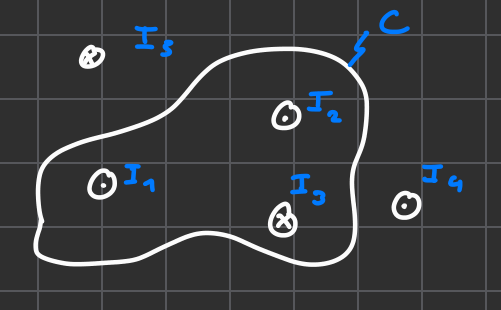
\includegraphics[width=0.8\textwidth]{images/loi-ampere.png}
 \end{minipage}
 \subsubsection{Champ $\bm B$ d'un champ rectiligne}
 \begin{minipage}{0.4\textwidth}
	\centering
	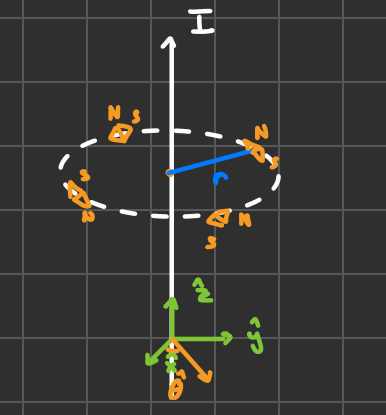
\includegraphics[width=0.6\textwidth]{images/ampere1.png}
\end{minipage}
\hfill
\begin{minipage}{0.6\textwidth}
	On considère un fil rectiligne infini portant un courant $I$ comme ci-près. L'expérience montre alors qu'un champ magnétique $\bm B$ est générée par le courant $I$ dans la direction $\theta$, orienté selon la règle de la main droite et de norme $B \propto \frac1r$. On trouve alors par calcul,
	\[
	\boxed{\bm B(\bm r) = \frac{\mu_0}{2 \pi r} I \bm e_\theta}
	\]
	où $\mu_0$ est la perméabilité du vide.
\end{minipage}
\subsubsection{Vers la loi d'Ampère}
\noindent
 \begin{minipage}{0.6\textwidth}
	On considère un fil rectiligne infini, on considère aussi le cercle $\gamma$ de rayon $r$ autour de $I$, ainsi
	\[
	\oint_\gamma \bm B \cdot \mathrm d \bm l = \int_0^{2\pi} B(r) \bm e_\theta \cdot \bm e_\theta \mathrm d \theta = B(r) r \int_0^{2\pi} \mathrm d \theta = \frac{\mu_0}{2 \pi r} I r 2 \pi = \mu_0 I
	\] 
	on remarque alors que le résultat est indépendant de $\bm r$
\end{minipage}
\hfill
\begin{minipage}{0.4\textwidth}
\centering
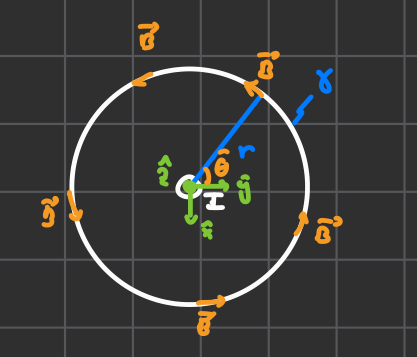
\includegraphics[width=0.6\textwidth]{images/ampere2.png}
\end{minipage}

\begin{minipage}{0.4\textwidth}
	\centering
	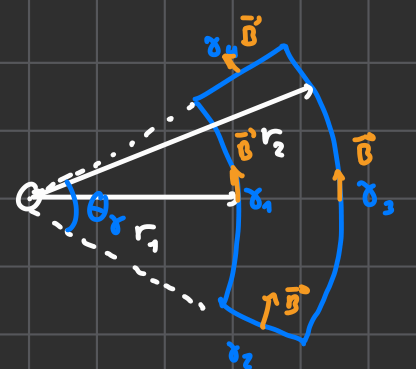
\includegraphics[width=0.6\textwidth]{images/ampere3.png}
	\vspace{0.5cm}
\end{minipage}
\hfill
\begin{minipage}{0.6\textwidth}
	Dans le cas où le chemin $\gamma$ ne passe pas autour de $I$, on trouve
	\begin{align*}
	\oint_\gamma \bm B \cdot \mathrm d\bm l &= \int_{\gamma_1} \bm B \cdot \mathrm d\bm l + \int_{\gamma_2} \bm B \cdot \mathrm d\bm l +\int_{\gamma_3} \bm B \cdot \mathrm d\bm l +\int_{\gamma_4 } \bm B \cdot \mathrm d\bm l \\
	&= - \frac{\mu_0 I}{2\pi r_1} r_1 \theta + 0 + \frac{\mu_0 I}{2 \pi r_2} r_2\theta + 0 \\
	&= - \frac{\mu_0 I}{2 \pi} \theta  + \frac{\mu_0 I}{2 \pi} \theta  = 0
	\end{align*}
\end{minipage}
On peut alors montrer que pour les chemins fermés arbitraire
\[
\oint_\gamma \bm B \cdot \mathrm d \bm l = \pm \mu_0 I \ou \oint_\gamma \bm B \cdot \mathrm d \bm l = 0
\]
selon si $\gamma$ entour le fil (une fois) ou pas. De plus, le \emph{principe de superposition} s'applique pour $\bm B$, donc pour un contour $\gamma$ quelconque pour des courants $I_m$, on a
\[
\oint_C \bm B \cdot \mathrm d \bm l = \mu_0 \sum I_m
\]

\subsubsection{Généralisation de la loi d'Ampère intégrale et différentielle locale}
Les règles précédentes restent valable pour des courants \emph{non-rectilignes}
\begin{figure}[H]
\centering
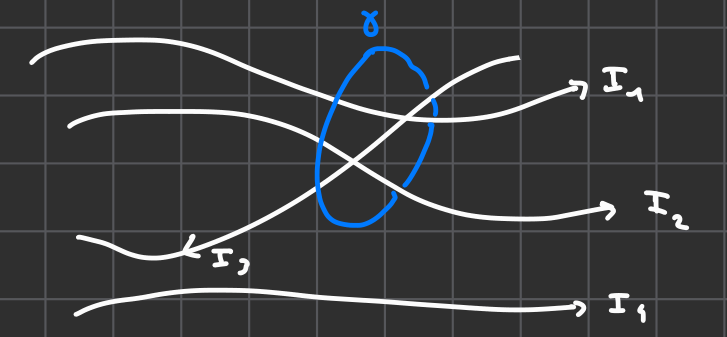
\includegraphics[width=0.3\textwidth]{images/ampere4.png}
\end{figure}
on a alors $\oint_\gamma \bm B \cdot \mathrm d \bm l = \mu_0 (I_1 + I_2 - I_3)$. Dans le cas d'une densité de courant $\bm I$, on a
\[
\boxed{\oint_\gamma \bm B \cdot \mathrm d \bm l = \mu_0 \iint_S \bm j \cdot \mathrm d \bm S}
\]
ou sinon par Stokes
\[
\oint_\gamma \bm B \cdot \mathrm d \bm l = \mu_0 \int_S \bm j \cdot \mathrm d \bm S \implies \iint_S (\nabla \times \bm B - \mu_0 \bm j) \cdot \mathrm d \bm S = 0
\]
et donc on conclut que
\[
\boxed{\nabla \times \bm B = \mu_0 \bm j}
\]
\subsection{Loi de Gauss pour \textit{B}}
	\noindent
	\begin{minipage}{0.6\textwidth}
			Contrairement au champ électrique, les lignes du champ $\bm B$ se sont jamais interrompus. Ainsi il n'y a pas de génération de lignes $\bm B$ pour tout $S$ fermé, ainsi
			 \[
			 \forall S \quad \iint_S \bm B \cdot \mathrm d\bm S = 0 \implies \forall V, \quad \iiint_V \nabla \cdot \bm B \mathrm dV = 0
			 \]
			 On en déduit donc que
			 \[
			 \boxed{\nabla \cdot \bm B = 0}
			 \]
	\end{minipage}
	\hfill
	\begin{minipage}{0.4\textwidth}
		\centering
		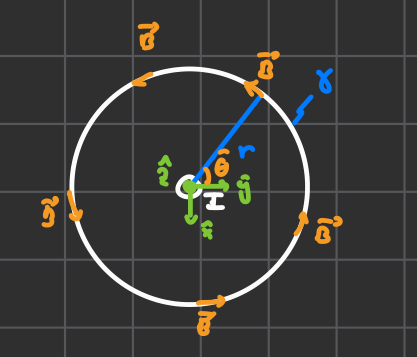
\includegraphics[width=0.6\textwidth]{images/ampere2.png}
	\end{minipage}
	
\subsection{Loi de Brot-Savart}
Quel est le champ $\bm B$ crée par une fil mince de forme arbitraire parcouru par un courant $I$?

Par ce qui précède on a
\[
\nabla \cdot \bm B = 0 \et \nabla \times \bm B = \mu_0 \bm j \implies \mathrm d \bm B(\bm p) =  \frac{\mu_0 I}{4 \pi} \frac{\mathrm d \bm l \times \bm r}{\norme{\bm r}^3}
\]
et donc le champ $\bm B$ crée par un fil mince arbitraire est donné par
\[
\boxed{\bm B(\bm p) = \frac{\mu_0 I}{4\pi} \int_{fil} \frac{\mathrm d \bm l \times \bm r}{\norme{\bm r}^3}}
\]
\subsection{Récapitulation des lois de l'électrostatique et de la magnétostatique}
Parmi toutes les équations que l'on a vu, On se pose alors la question les quelles sont encore valable dans un cardre dynamique. La réponse est
\[
\nabla \cdot E = \frac{\rho_{el}}{\varepsilon_0}, \quad \nabla \cdot B = 0 \et \bm F = q (\bm E + \bm v \times \bm B)
\]
Tandis que celles-ci ne sont plus valable dans un cadre dynamique
\[
\nabla \times E = 0 \et \nabla \times B = \mu_0 \bm j
\]

\clearpage

\section{Phénomènes d'induction magnétique}
\subsection{Loi d'induction de Faraday}
On considère le système
\begin{figure}[H]
	\centering
	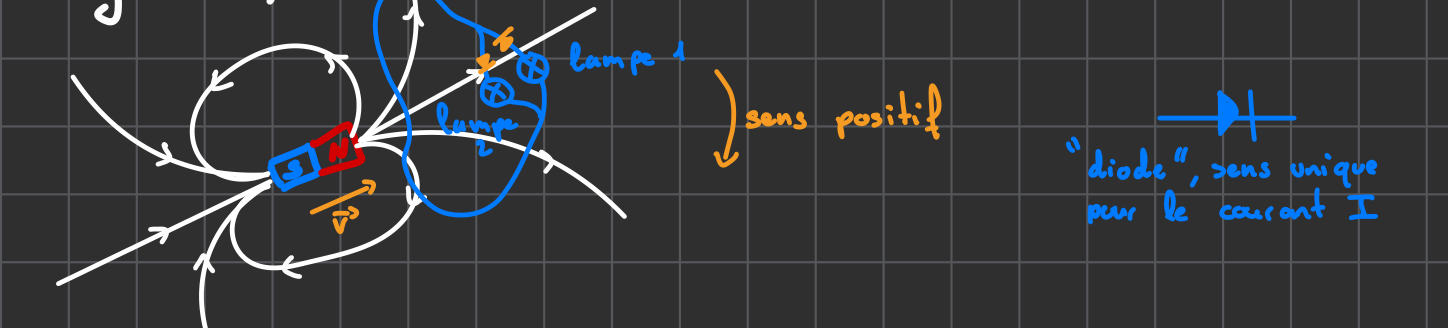
\includegraphics[width=0.6\textwidth]{images/induction-faraday.png}
\end{figure}
On remarque la présence d'un champ électrique, or on sait que
\[
\bm j = \frac{I}{S}\frac{\mathrm d \bm l}{\mathrm dl} \et \bm j = \sigma_c \bm E \implies \bm E = \frac{I}{S \sigma_c} \frac{\mathrm d \bm l}{\mathrm dl}
\]
ainsi
\[
\oint_{fil} \bm E \cdot \mathrm  d \bm l = \frac{I}{S \sigma_c} \oint_{fil} \frac{\mathrm d \bm l}{\mathrm dl} \cdot \mathrm d \bm l = \frac{I}{S \sigma_c} \oint_{fil} \mathrm dl = \frac{Il}{s \sigma_c} = I R \neq 0
\]
donc $\oint \bm E \cdot \mathrm d \bm l \neq 0$ \footnote{donc on ne peut plus écrire $\bm E = - \nabla \phi$, car sinon on aurait $0 \neq 0$ en utilisant stokes} en générale. On appelle $\varepsilon_{ind}$ la \emph{tension induite} ou \emph{force électromotrice induite}. Cette FEM est induite par le mouvement de l'aimant. On en déduit que le phénomène est dû à la \textbf{variation} du champ magnétique au cours du temps (plus précisement c'est la variation du flux de $\bm B$). Une expérience montre quantitative, nous montre que
\[
\boxed{\varepsilon_{ind} = \oint_{fil} \bm E \cdot \mathrm d \bm l = - \frac{\mathrm d}{\mathrm d t} \iint_S \bm B \cdot \mathrm d \bm S = - \frac{\mathrm d }{\mathrm dt} \Phi}
\]
où $\phi$ correspond au \emph{flux du champ} $\bm B$ à travers $S$. 

\subsection{Loi de Faraday différentielle}
Par ce qui précède on a que
\[
\oint_\gamma \bm E \cdot \mathrm d \bm l = - \frac{\mathrm d}{\mathrm dt} \iint_S \bm B \cdot \mathrm \bm S = - \iint_S \frac{\partial \bm B}{\partial t} \cdot \mathrm d \bm S
\]
En plus, par stokes on a
\[
\oint_\gamma \bm E \cdot \mathrm d \bm l = \iint_S \nabla \times \bm E \cdot \mathrm d \bm S
\]
On peut donc en conclure, par arbitrarité de $\gamma$ que 
\[
\boxed{\nabla \times E = - \frac{\partial \bm B}{\partial t}}
\]
\clearpage
\subsection{Règle de Lenz}
Il est important de déterminer quel est la direction du courant (et du champ $\bm E$) induit. La réponse est donné par le règle de Lenz : 

\textit{"Le courant induit $I$ dans la boucle est orienté tel que le champ $\bm B$ qu'il crée lui s'oppose au chamgement du flux mangétique."}

\subsection{Circuit électrique en présence de phénomènes d'induction}
\subsubsection{Self-induction}

\begin{wrapfigure}{r}{0.4\textwidth}
	\centering
	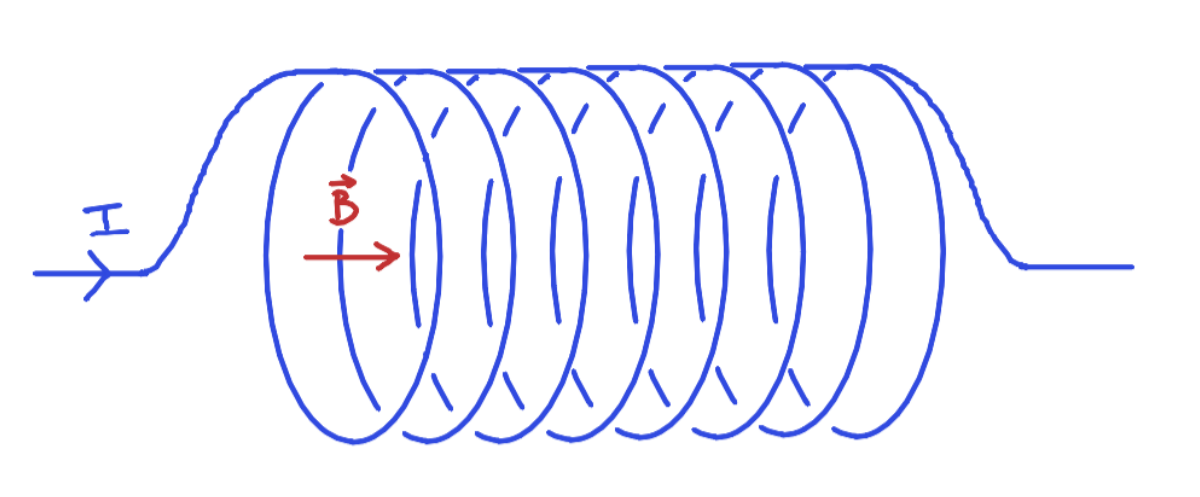
\includegraphics[width=0.3\textwidth]{images/bobine.png}
\end{wrapfigure}
	Si on considère une bobine comme ci-près, on a $B \simeq \mu_0 In$ à l'intérieur de la bobine, où $n$ est le nombre de tours par mètre. Ce $B$ produit un flux $\Phi$ à travers la bobine elle même. Ainsi par boucle on a $\Phi = BS = \mu_0 In S$. Or la bobine est le loungueur $l$ et à $n \cdot l$ boucle, ainsi
\[
\Phi_{tot} = \Phi nl = \mu_0 n^2 ls I = LI
\]
avec $L:= \mu_0 n^2 l S$ l'\emph{l'auto-inductance} ou \emph{self} de la bobine. L'unité est $[L] = \unit{T.m^2.A^{-1}} = \unit{H}$. Ainsi si $\dot I \neq 0$ alors $\dot \Phi \neq 0$, donc une bobine induit une tension dans elle même, ainsi
\[
\boxed{\varepsilon_{ind} = -\dot \Phi = - L \dot I}
\]

\subsubsection{Circuit électrique avec un self}
Si on considère le circuit comme ci-près, par la loi des mailles de Kirchhoff on trouve que 
\begin{wrapfigure}{l}{0.4\textwidth}
	\centering
	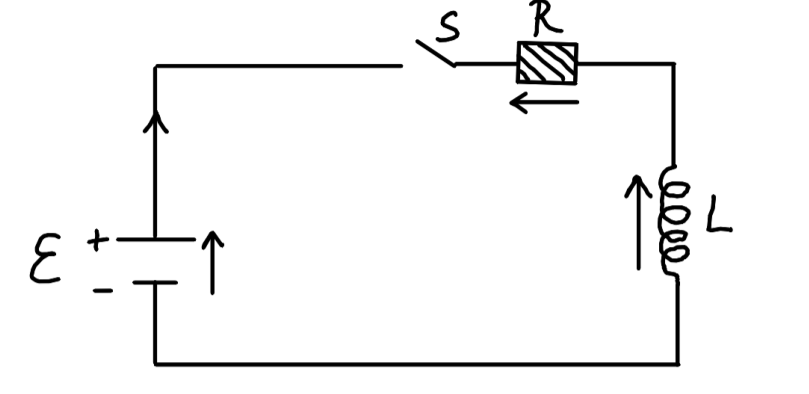
\includegraphics[width=0.3\textwidth]{images/circuit-bobine.png}
	\caption{Cicuit électrique avec un self}
	\label{fig: circuit avec self}
\end{wrapfigure}
\[
L \dot I + RI = \varepsilon
\]
on a alors une équation différentielle linéaire d'ordre $1$ ayant comme condition initiale $I(0) = 0$, on trouve donc
\[
I(t) = \frac{\varepsilon}{R} (1 - e^{- \frac{R}{L} t})
\]
On remarque alors qu'un self a tendance à ralentir de courant.

\subsubsection{Signe de $\varepsilon_{ind}$ dans la loi de Maille}
On se demande lorsque qu'on applique la loi des mailles contentant une tensions induite $\varepsilon_{ind}$ comment savoir savoir quelle est le signe mettre.

Si l'on choisit une orientation pour $\mathrm d \bm S$ tel que $I$ circule le sens respectant la règle de la main droite, alors cela donnera un signe $+$ à $\varepsilon_{ind}$.

\subsubsection{Énergie mécanique}
Si l'on se rappelle de l'équation différentielle dans l'exemple \eqref{fig: circuit avec self} on a
\[
\varepsilon = L \dot I + R I
\]
et donc en multipliant de part et autre par $I$ on obtient 
\[
\boxed{\varepsilon I = R I^2 + I L\dot I}
\]
On peut alors noté que $\varepsilon I$ correspond à l'énergie fournie par le FEM, que $RI^2$ correspond à la puissance dissipée par effet Joule et finalement $IL\dot I$ est la puissance nécessaire pour que les charges puisse surmonter la tension induite.

On note que la puisse $I L \dot I$ est stocké dans le champ $\bm B$ de la bobine en forme d'énergie magnétique, on peut alors calculer cette énergie
\[
W_{self} = \int_0^{t_0}	P \mathrm d t = \int_0^{t_0} I L  \dot I \mathrm dt = \frac12 L(I^2(t_0) - I^2(0)) = \frac12L I_0^2
\]
et donc dans le cas où on a une bobine solénoïde idéale : $L = \mu_0 n^2 l S$ et $I = \frac{B}{\mu_0 n}$, alors
\[
W_{self} = \frac12 L I^2 = \frac{B^2}{2 \mu_0} lS
\]
où $ls$ correspond au volume $V$ entouré par le bobine. Alors la \emph{densité d'énergie mécanique} vaut
\[
e_B = \frac12 \frac{B^2}{\mu_0}
\]
Ce qui permet de trouver la densité d'énergie électrique et magnétique dans le vide 
\[
\boxed{e_{EB} = e_E + e_B = \frac12 \varepsilon_0 E^2 + \frac12 \frac{B^2}{\mu_0}}
\]

\clearpage
\section{Équations de Maxwell}
\subsection{Critique de l'équation d'Ampère $\nabla \times B = \mu_0 j$.}
En générale, la loi d'Ampère $\nabla \times \bm B = \mu_0 \bm j$ n'est pas valable. En effet comme
\[
\nabla \cdot (\nabla \times \bm B) = 0
\]
et donc en prenant la divergence de la loi d'Ampère on obtient $\nabla \cdot \bm j = 0$. En injectant alors ceci dans l'équation de continuité on trouve
\[
\frac{\partial \rho_{el}}{\partial t} = 0 
\]
Mais ceci est certainement faux en générale.

\subsection{Courant de déplacement de Maxwell}
James Maxwell avait postulé qu'un terme supplémentaire étant nécessaire dans la loi d'Ampère dans le cadre plus générale de la dynamique
\[
\boxed{\nabla \times \bm B = \mu_0 \bm j + \mu_0 \varepsilon_0 \frac{\partial \bm E}{\partial t}}
\]
où $\varepsilon_0 \frac{\partial \bm E}{\partial t}$ a les unités d'une densité de courant. Il est appelé \emph{densité de courant de déplacement}.

De cette loi, on en tire facilement une forme intégrale. Pour un chemin $\gamma$ fermé arbitraire on a
\[
\oint_\gamma \bm B \cdot \mathrm d \bm S = \iiint_S \nabla \times \bm B \cdot \mathrm d \bm S = \iint_S \left(\mu_0 \bm j + \mu_0 \varepsilon_0 \frac{\partial \bm E}{\partial t} \right) \cdot \mathrm d \bm S
\]
ainsi on a la loi d'Ampère-Maxwell
\[
\oint_\gamma \bm B \cdot \mathrm d \bm S = \iint_S \left(\mu_0 \bm j + \mu_0 \varepsilon_0 \frac{\partial \bm E}{\partial t} \right) \cdot \mathrm d \bm S
\]
\subsection{Les équations de Maxwell}
On obtient alors le système d'équation suivant
\[
\nabla \cdot \bm E = \frac{\rho_{el}}{\varepsilon_0}, \quad \nabla \times \bm E = - \frac{\partial \bm B}{\partial t}, \quad \nabla \cdot \bm B = 0, \quad \nabla \times \bm B = \mu_0 \bm j + \mu_0 \varepsilon_0 \frac{\partial \bm E}{\partial t}
\]
Les équations de Maxwell décrivent, entre autre, que les charges et les courants sont sources des champs électromagnétique ($\bm E$ et $\bm B$). En revanche, la force exercée par $\bm E$ et $\bm B$ sur une charge est donnée par
\[
\bm F = q(\bm E + \bm v \times \bm B)
\]
\end{document}






